%% Version 6.1, 1 September 2021
%
%%%%%%%%%%%%%%%%%%%%%%%%%%%%%%%%%%%%%%%%%%%%%%%%%%%%%%%%%%%%%%%%%%%%%%
% TemplateV6.1.tex --  LaTeX-based blank template for submissions to the 
% American Meteorological Society
%
%%%%%%%%%%%%%%%%%%%%%%%%%%%%%%%%%%%%%%%%%%%%%%%%%%%%%%%%%%%%%%%%%%%%%
% PREAMBLE
%%%%%%%%%%%%%%%%%%%%%%%%%%%%%%%%%%%%%%%%%%%%%%%%%%%%%%%%%%%%%%%%%%%%%

%% Start with one of the following:
% 1.5-SPACED VERSION FOR SUBMISSION TO THE AMS
\documentclass{ametsocV6.1}

% TWO-COLUMN JOURNAL PAGE LAYOUT---FOR AUTHOR USE ONLY
% \documentclass[twocol]{ametsocV6.1}

%%%%%%%%%%%%%%%%%%%%%%%%%%%%%%%%

%%% To be entered by author:

%% May use \\ to break lines in title:

\title{Static and dynamic performance of the RBR\textit{argo}$^3$ CTD}

%% Enter authors' names and affiliations as you see in the examples below.
%
%% Use \correspondingauthor{} and \thanks{} (\thanks command to be used for affiliations footnotes, 
%% such as current affiliation, additional affiliation, deceased, co-first authors, etc.)
%% immediately following the appropriate author.
%
%% Note that the \correspondingauthor{} command is NECESSARY.
%% The \thanks{} commands are OPTIONAL.
%
%% Enter affiliations within the \affiliation{} field. Use \aff{#} to indicate the affiliation letter at both the
%% affiliation and at each author's name. Use \\ to insert line breaks to place each affiliation on its own line.

%\authors{Author One,\aff{a}\correspondingauthor{Author One, email@email.com} 
%Author Two,\aff{a} 
%Author Three,\aff{b} 
%Author Four,\aff{a} 
%Author Five\thanks{Author Five's current affiliation: NCAR, Boulder, Colorado},\aff{c} 
%Author Six,\aff{c} 
%Author Seven,\aff{d}
% and Author Eight\aff{a,d}
%}
%
%\affiliation{\aff{a}{First Affiliation}\\
%\aff{b}{Second Affiliation}\\
%\aff{c}{Third Affiliation}\\
%\aff{d}{Fourth Affiliation}
%}

\authors{M. Dever\aff{a,b}\correspondingauthor{M. Dever, mathieu.dever@rbr-global.com},
B. Owens\aff{b},
C. Richards\aff{c},
S. Wijffels\aff{b},
A. Wong\aff{d},
I. Shkvorets\aff{a},
M. Halverson\aff{a},
G. Johnson\aff{a}
}

\affiliation{\aff{a}{RBR, Ottawa, Canada}\\
\aff{b}{Woods Hole Oceanographic Institution, Woods Hole, USA}\\
\aff{c}{Bedford Institute of Oceanography, Department of Fisheries and Oceans Canada, Dartmouth, Canada}\\
\aff{d}{School of Oceanography, University of Washington, Seattle, WA, USA}
}

%%%%%%%%%%%%%%%%%%%%%%%%%%%%%%%%%%%%%%%%%%%%%%%%%%%%%%%%%%%%%%%%%%%%%
% ABSTRACT
%
% Enter your abstract here
% Abstracts should not exceed 250 words in length!
%
 
\abstract{The static and dynamic performances of the RBR\textit{argo}$^3$ are investigated using a combination of lab-based and in situ datasets from floats deployed in an Argo Program pilot program.  Long term deployments show no significant drift in salinity. Static accuracy of salinity is significantly improved using (1) a time lag for temperature, (2) a quadratic pressure dependence and (3) by laboratory calibrating each RBR\textit{argo}$^3$ for a range of pressures. The presence of two different adjustment timescales is unravelled: a long-term adjustment O(120 s), driven by the temperature difference between the interior of the conductivity cell and the water, and a short-term adjustment O(5-10 s), associated by the initial exchange of heat between the water and the inner ceramic.  Corrections for these effects, including dependence on
profiling speed are developed. The strong speed dependence of the dynamic corrections suggests that profiling at higher speeds ($>$ 15 cm/s) would help minimize dynamic errors. }

\begin{document}

%% Necessary!
\maketitle

%%%%%%%%%%%%%%%%%%%%%%%%%%%%%%%%%%%%%%%%%%%%%%%%%%%%%%%%%%%%%%%%%%%%%
% MAIN BODY OF PAPER
%%%%%%%%%%%%%%%%%%%%%%%%%%%%%%%%%%%%%%%%%%%%%%%%%%%%%%%%%%%%%%%%%%%%%
%

\section{Introduction}
Diversification of Conductivity-Temperature-Depth (CTD) instrumentation for the Argo program is crucial to avoid "points of single failure" \citep{Roemmich_2019}. As an alternative CTD to the one currently used on Argo floats, the RBR\textit{argo}$^3$, manufactured by RBR Ltd., was approved for a trial phase to assess its in-situ performance. Several floats equipped with the RBR\textit{argo}$^3$ have thus been deployed and a task team with members from  the Argo community and RBR formed in 2020 to assess instrument accuracy across a range of ocean regimes, help improve calibrations, and develop the procedures to yield the highest data quality. 

The RBR\textit{argo}$^3$ conductivity cell relies on a different working principle than the SBE41CP CTD currently used on Argo floats, which relies on an electrode-based measurement of conductivity within a borosilicate glass cell through which water is actively and continuously pumped \citep{Lueck_1990a}. The RBR\textit{argo}$^3$, on the other hand, uses a free-flushing, low aspect ratio conductivity cell \citep[Figure \ref{fig: RBRargo3};][]{Halverson_2020}. Conductivity measurements of the seawater in the vicinity of the cell are made according to Faraday’s law of induction, using two toroidal coils -- a generating coil and a receiving coil. An alternating voltage is applied to the generating coil, producing a time-varying magnetic field and thereby inducing a current in the seawater inside and surrounding the cell (Figure \ref{fig: RBRargo3}). The induced current loops through the seawater and passes through the center of the receiving coil, generating a secondary current. The measured current in the receiving coil is proportional to the conductivity of the seawater.

\begin{figure}[t]
	\centering
	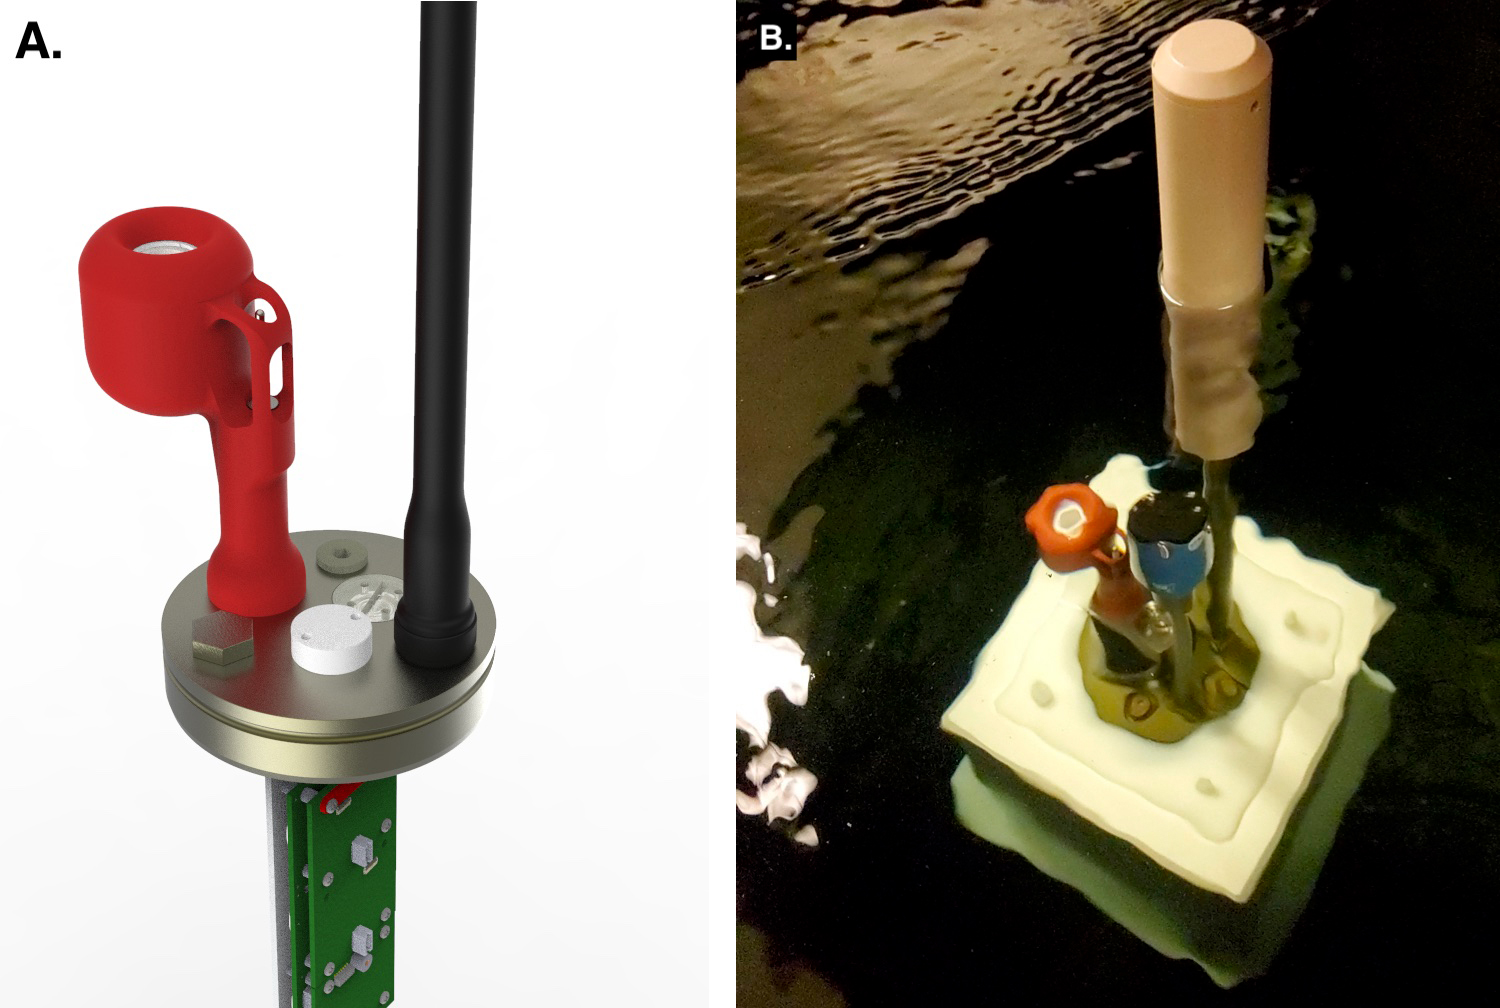
\includegraphics[width = .95\linewidth]{Fig1}
	\caption{(\textbf{A.}) Rendering of an RBR\textit{argo}$^3$ mounted on an Argo float cap.  (\textbf{B.}) Photo of the RBR\textit{argo}$^3$ mounted on an Argo float during calibration (credits Kai Malorny).}
	\label{fig: RBRargo3}
\end{figure}

The static accuracy at sea-level of the RBR\textit{argo}$^3$ is stated to be $\pm$ 0.003 mS/cm, $\pm$ 0.002 $^{\circ}$C, and $\pm$ 1 dbar for conductivity, temperature, and pressure, respectively. 
However, compressibility effects can affect the static accuracy of conductivity at high pressures, and sensor drift can degrade the static accuracy of conductivity measurements over time. 
The profiling nature of Argo floats also generate dynamic errors in CTD observations \citep{Lueck_1990b, Morison_1994,Johnson_2007}. 
In fact, dynamic errors emerge in CTD observations when collected from any moving platform sampling through a temperature gradient, and are proportional to the amplitude of the temperature gradient. 
These dynamic errors are generated by different processes linked to the physical arrangement of the sensors, the inherent response time of the sensors, and the thermal inertia of the conductivity cell.

In this study, each of these sources of error are characterized and post-processing techniques are developed to correct these errors in order to improve the resulting data accuracy. 

\section{Theoretical Framework}
\label{sec: theory}
\subsection{Static-accuracy and compressibility correction}
Static accuracy of the RBR\textit{argo}$^3$ is determined during the calibration process at RBR, and detailed on the calibration certificate provided with each RBR\textit{argo}$^3$.
Instrument calibration is typically performed at atmospheric pressure. 
At higher pressure, however, the geometry of the conductivity cell on the RBR\textit{argo}$^3$ elastically deforms, changing the path of the current in the sampled seawater, and therefore introducing a pressure-dependent bias in the conductivity measurements.  This compressibility error is expected to be repeatable from profile to profile and to vary for each CTD (see Section 4). 

\subsection{Sensor stability}
Each float deployed as part of the Argo program is expected to have a life expectancy of a minimum of 5 years. 
Sensors onboard floats must therefore demonstrate not only good stability from profile-to-profile, but also over timescales on the order of years.
Salinity drift is one of the main challenges the Argo program faces \citep{Wong_2020}.  
Stability of salinity estimates from Argo floats can be affected by many different factors, including biofouling, biocide leakage, or degradation of the cell over time such as deformation or seawater penetration \citep{Wong_2003, Wong_2020}.  Assessing long term stability does require `ageing' the sensor on an float following an Argo mission, during which the CTD is at 1000 dbar for 90\% of its lifetime.

\subsection{Dynamic errors and their impact on salinity estimation}
Conductivity in the ocean is to first order dominated by temperature, with salinity a relatively minor  player. Thus any mismatch between simultaneous temperature and conductivity measurements used to estimate salinity can generate large errors.   
For a profiling CTD, two types of dynamic errors affect salinity estimates: (1) a time lag between temperature and conductivity measurements and (2) a temperature difference between the fluid at the thermistor and in the measurement volume of the conductivity cell due to its larger thermal inertia \citep{Lueck_1990a,Johnson_2007}. 
Both of these dynamic errors can be observed in-situ and are especially obvious when a CTD profiles through a temperature interface into a relatively homogeneous layer, which typically occur in regions of double-diffusive instability or near the base of the surface mixed layer. 
Figure \ref{fig: alamo_example} shows an example profile collected by an RBR\textit{argo}$^3$ -equipped ALAMO float in the Caribbean Sea, where both the salinity and the potential density anomaly clearly exhibit artificial features at temperature interfaces \citep{Jayne_2017, Sanabia_2020}. 
The error in salinity (and potential density) has both a short time scale, O(5-10 sec), seen as a high salinity/density spike near the lower boundary of the well-mixed layer, and a longer time scale O(120 seconds) that extends over much of the mixed-layers and is best visible as an artificial negative slope in the potential density as a function of pressure.

\begin{figure}[t]
	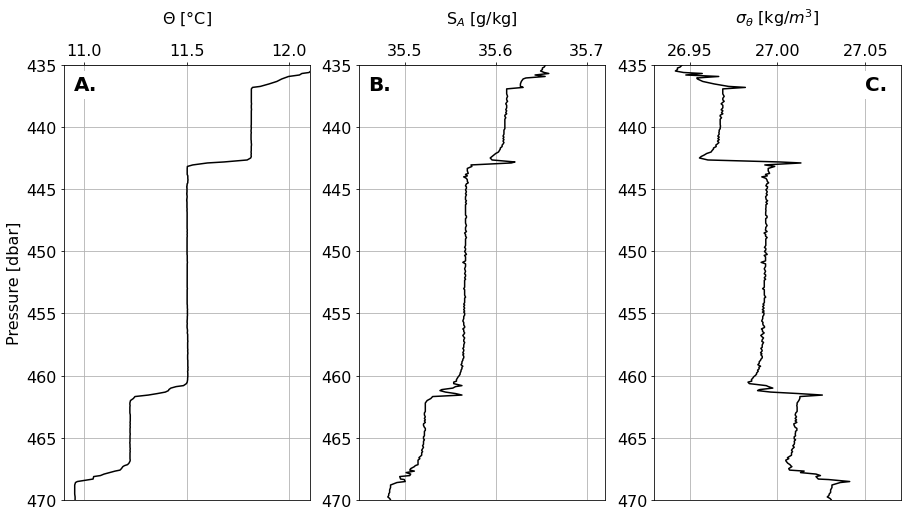
\includegraphics[width = \linewidth]{Fig2_f9139_P52.png}
	\caption{Example profile from ALAMO float 9139 in the Caribbean Sea (profile 52), showing (\textbf{A.}) the conservative temperature, (\textbf{B.}) the absolute salinity, and (\textbf{C.}) the potential density anomaly. The staircase structure of the water column highlights dynamic errors in both salinity and density at sharp interfaces, where both spiking and thermal inertia errors can be seen. Data Courtesy of Drs Sanabia (US Naval Academy) and Jayne (Woods Hole Oceanographic Institution).}
	\label{fig: alamo_example}
\end{figure}

\subsubsection{Response time and sensor misalignments}
Misalignments between temperature and conductivity measurements generate errors in salinity estimates, often called ``salinity spiking" \citep{Horne_1980,Ullman_2014,Dever_2020}. This misalignment is referred to as a ``C-T lag", and is generated by two separate mechanisms:
\begin{enumerate}
	\item The physical separation between the thermistor and the conductivity cell. As it takes time for the sampled water parcel to travel from the thermistor to the volume sampled by the conductivity cell, this "advective lag" is directly proportional to the distance between the thermistor and the conductivity cell, and is therefore dependent on the flow speed through the CTD. The RBR\textit{argo}$^3$ CTD has been designed to minimize the spatial separation between conductivity and temperature, and thus the advective C-T lag (see Figure \ref{fig: RBRargo3}).
	\item The inherent response time of the thermistor. The thermistor responds more slowly to a change in temperature than the conductivity cell who is virtually instantaneous due to the fact that it is an electrical measurement and does not rely on diffusion processes the way the thermistor does. This difference in response time introduces an apparent time-lag between the temperature and conductivity, resulting in spiking in the computed salinity \citep{Horne_1980}. This C-T lag is caused by the inherent properties of the thermistor and can be considered to be independent of flow-speed to the first degree of approximation.
\end{enumerate}

This error can be seen in Figure \ref{fig: alamo_example}, with some evident salinity spiking coinciding with sharp temperature gradients, and can be corrected by shifting the measured temperature in time using:

\begin{equation}
T_{cor}(t) = T_{meas}(t + \Delta t)
\label{eq: CTlag}
\end{equation}
where $T_{cor}$ is the lagged temperature, $T_{meas}$ is the raw temperature, and $\Delta$t is the prescribed lag. Other approaches than a simple time-lag are sometimes considered to correct for the C-T lag, such as sharpening algorithms \citep{Fozdar_1985, Bittig_2014,Johnson_2007}. Sharpening algorithms present the advantage to further reduce the salinity spiking by reconstructing fine-scale gradients that are not captured by the sensor.  However, the reliability of all these techniques depends on both the amplitude and phase reconstruction.  The time-lag approach was deemed to be a good compromise between phase and amplitude reconstruction of the signal across the frequency range. 

\subsubsection{Thermal inertia errors}
\label{sec: plunging}

As the CTD travels through a temperature gradient, heat is exchanged between the conductivity cell and a thin boundary layer attached to the cell, which changes the temperature averaged over the conductivity measurement volume from that measured by the thermistor.
Thus, the calculated salinity must use a temperature adjusted for the heat flux into the measurement volume.
This is a well-known, but poorly constrained, error in CTD measurements generally, and is the focus of a research effort that has been ongoing for over three decades \citep{Lueck_1990b, Morison_1994, Johnson_2007, Martini_2019, Johnson_2020, Halverson_2020}.
As described by Lueck (1990), the heat flux at the cell boundary will depend on the profiling speed and the difference between the cell surface temperature and $T_{cor}$ while the thickness of the boundary layer which determines the contribution to the measurement averaged temperature will depend on the profiling speed.
The surface temperature of cell will depend on the heat conduction within the cell.

While the transfer of heat into the fluid depends on the skin temperature of the cell, the change in the skin temperature will depend on the thermal conductance of the cell components.  
As shown in Figure \ref{fig: RBRargo3}, the cell is constructed from materials for which the thermal conductance varies by more than a factor of 20.

In a cylindrical coordinate system, the equation describing the diffusion of heat can be written as:

\begin{equation}
\rho C_p \frac{\partial T}{\partial t} = \frac{1}{r}\frac{\partial}{\partial r}\left(r\lambda\frac{\partial T}{\partial r}\right)
\label{eq: heat_conduction}
\end{equation}
where $\rho$ is the density of the material, $C_p$ is the heat capacity, T is the temperature inside the conductivity cell,  $r$ is the distance from the center of the ceramic annulus (see Figure \ref{fig: RBRargo3}), and $\lambda$ is the thermal conductivity.

After a short time the heat content of material near the cell boundary changes slowly, so that the left hand side of Equation \ref{eq: heat_conduction} approaches zero. Thus for longer timescales the heat conductance into the cell can be approximated using the average thermal conductance and the difference between the temperature measured inside the cell which must equal the heat flux through the surface boundary layer. This approximate balance leads to an expression for the temperature anomaly at long time scales:

\begin{equation}
%	\frac{C_{cor}}{C_{meas}} - 1 = \text{ctcoeff} \times (T_{cond} - T_{cor})
	T_{long} = \text{ctcoeff (V}_p) \times (T_{cond} - T_{cor})
	\label{eq: long-term_TM}
\end{equation}
where $T_{long}$ is the temperature anomaly in the sampled volume due to long-term thermal inertia, $T_{cond}$ is the internal temperature of the conductivity cell, $T_{cor}$ is the lagged temperature of the seawater, and $\text{ctcoeff}$ is a scaling coefficient that is a function of the profiling speed V$_p$.The profiling speed is defined as the velocity of the water at the CTD. 

On shorter timescales, the approach used to correct for thermal inertia errors has traditionally relied on an idealized model developed by \cite{Lueck_1990a} and slightly modified by \cite{Lueck_1990b} and \cite{Morison_1994}. 
The model, hereafter referred to as L\&P90, is essentially a recursive filter that aims to estimate the short-term temperature anomaly of the volume of water present in the conductivity cell as the CTD travels through a seawater temperature gradient. It relies on two key parameters, namely $\alpha$ and $\tau$, that drive the amplitude and timescale of the filter. It is expressed in discrete form using the following equation \citep{Morison_1994}:

\begin{align}
	\label{eq: LP}
%	T_{cell}(n) &= T_{cor}(n) - T_{adj}(n)\nonumber\\
	T_{short}(n) &= -b T_{short}(n-1) + a (T_{cor}(n) - T_{cor}(n-1))
\end{align}
where $T_{short}$ is the short-term temperature anomaly estimated by the filter, and $n$ is the index for a discrete measurement. The two coefficients $a$ and $b$ are computed using:

\begin{align}
	\label{eq: LP2}
	a &= \frac{4f_N\alpha\tau}{1+4f_N\tau}\nonumber\\
	b &= 1-\frac{2a}{\alpha}
\end{align}
where $f_N$ is the Nyquist frequency, and $\alpha$ and $\tau$ are empirically determined parameters (see section \ref{sec: results}).

The total estimated temperature of the sampled volume can be estimated by combining both of those temperature anomalies with the measured temperature:
\begin{equation}
T_{cell} = T_{cor} + T_{anomaly} = T_{cor} + T_{long} - T_{short} 
\end{equation}
where $T_{cell}$ is the estimated temperature of the sampled volume, corrected for both long- and short-term thermal inertia, and is used to derive the corrected salinity.

\section{Datasets and Methodology}
\label{sec: datasets}
\subsection{Static accuracy and compressibility correction}
\label{sec: static_datasets}
The static accuracy of temperature and pressure were assessed utilizing data from four ship-board campaigns (Table \ref{tab: cruise_data}), where RBR\textit{concerto}$^3$ CTDs, which use equivalent thermistors and pressure sensors as the RBR\textit{argo}$^3$, were mounted on CTD rosettes equipped with SBE9 CTDs. The latter typically had two pairs of SBE4 temperature sensors and pressure was measured by a Para-scientific quartz sensor. The SBE9 is powered via a cable to the ship and reports back 24 Hz data. The accuracy of the SBE9 system post calibration is 0.001$^\circ$C and 0.015\% range for pressure (0.3 dbar). The RBR CTDs on the rosettes were internally recording and were typically set to sample at 8 to 12 Hz.  A first gross comparison was made of the two SBE9 channels, and the primary was chosen for the temperature comparison below. 

To compare pressure readings, the SBE9 and RBR data streams were interpolated to the RBR's timebase, and then the cross-correlations function was computed  for pressure. 
The computed lags miximizing the cross-correlation function were then used to synchronize the data streams, exploiting the small (~1-2dbar) pressure changes associated with surface wave action on the CTD fall and rise rates. 
Once synchronized, the difference of the pressures was found, and then binned every 20 dbar (using the SBE9 pressure) across all 4 voyages and all RBR CTDs (Table \ref{tab: cruise_data}). 
In each 20 dbar bin, the distribution of pressure differences was calculated (Figure \ref{fig: PT_accuracy}). 

\begin{figure}[t]
	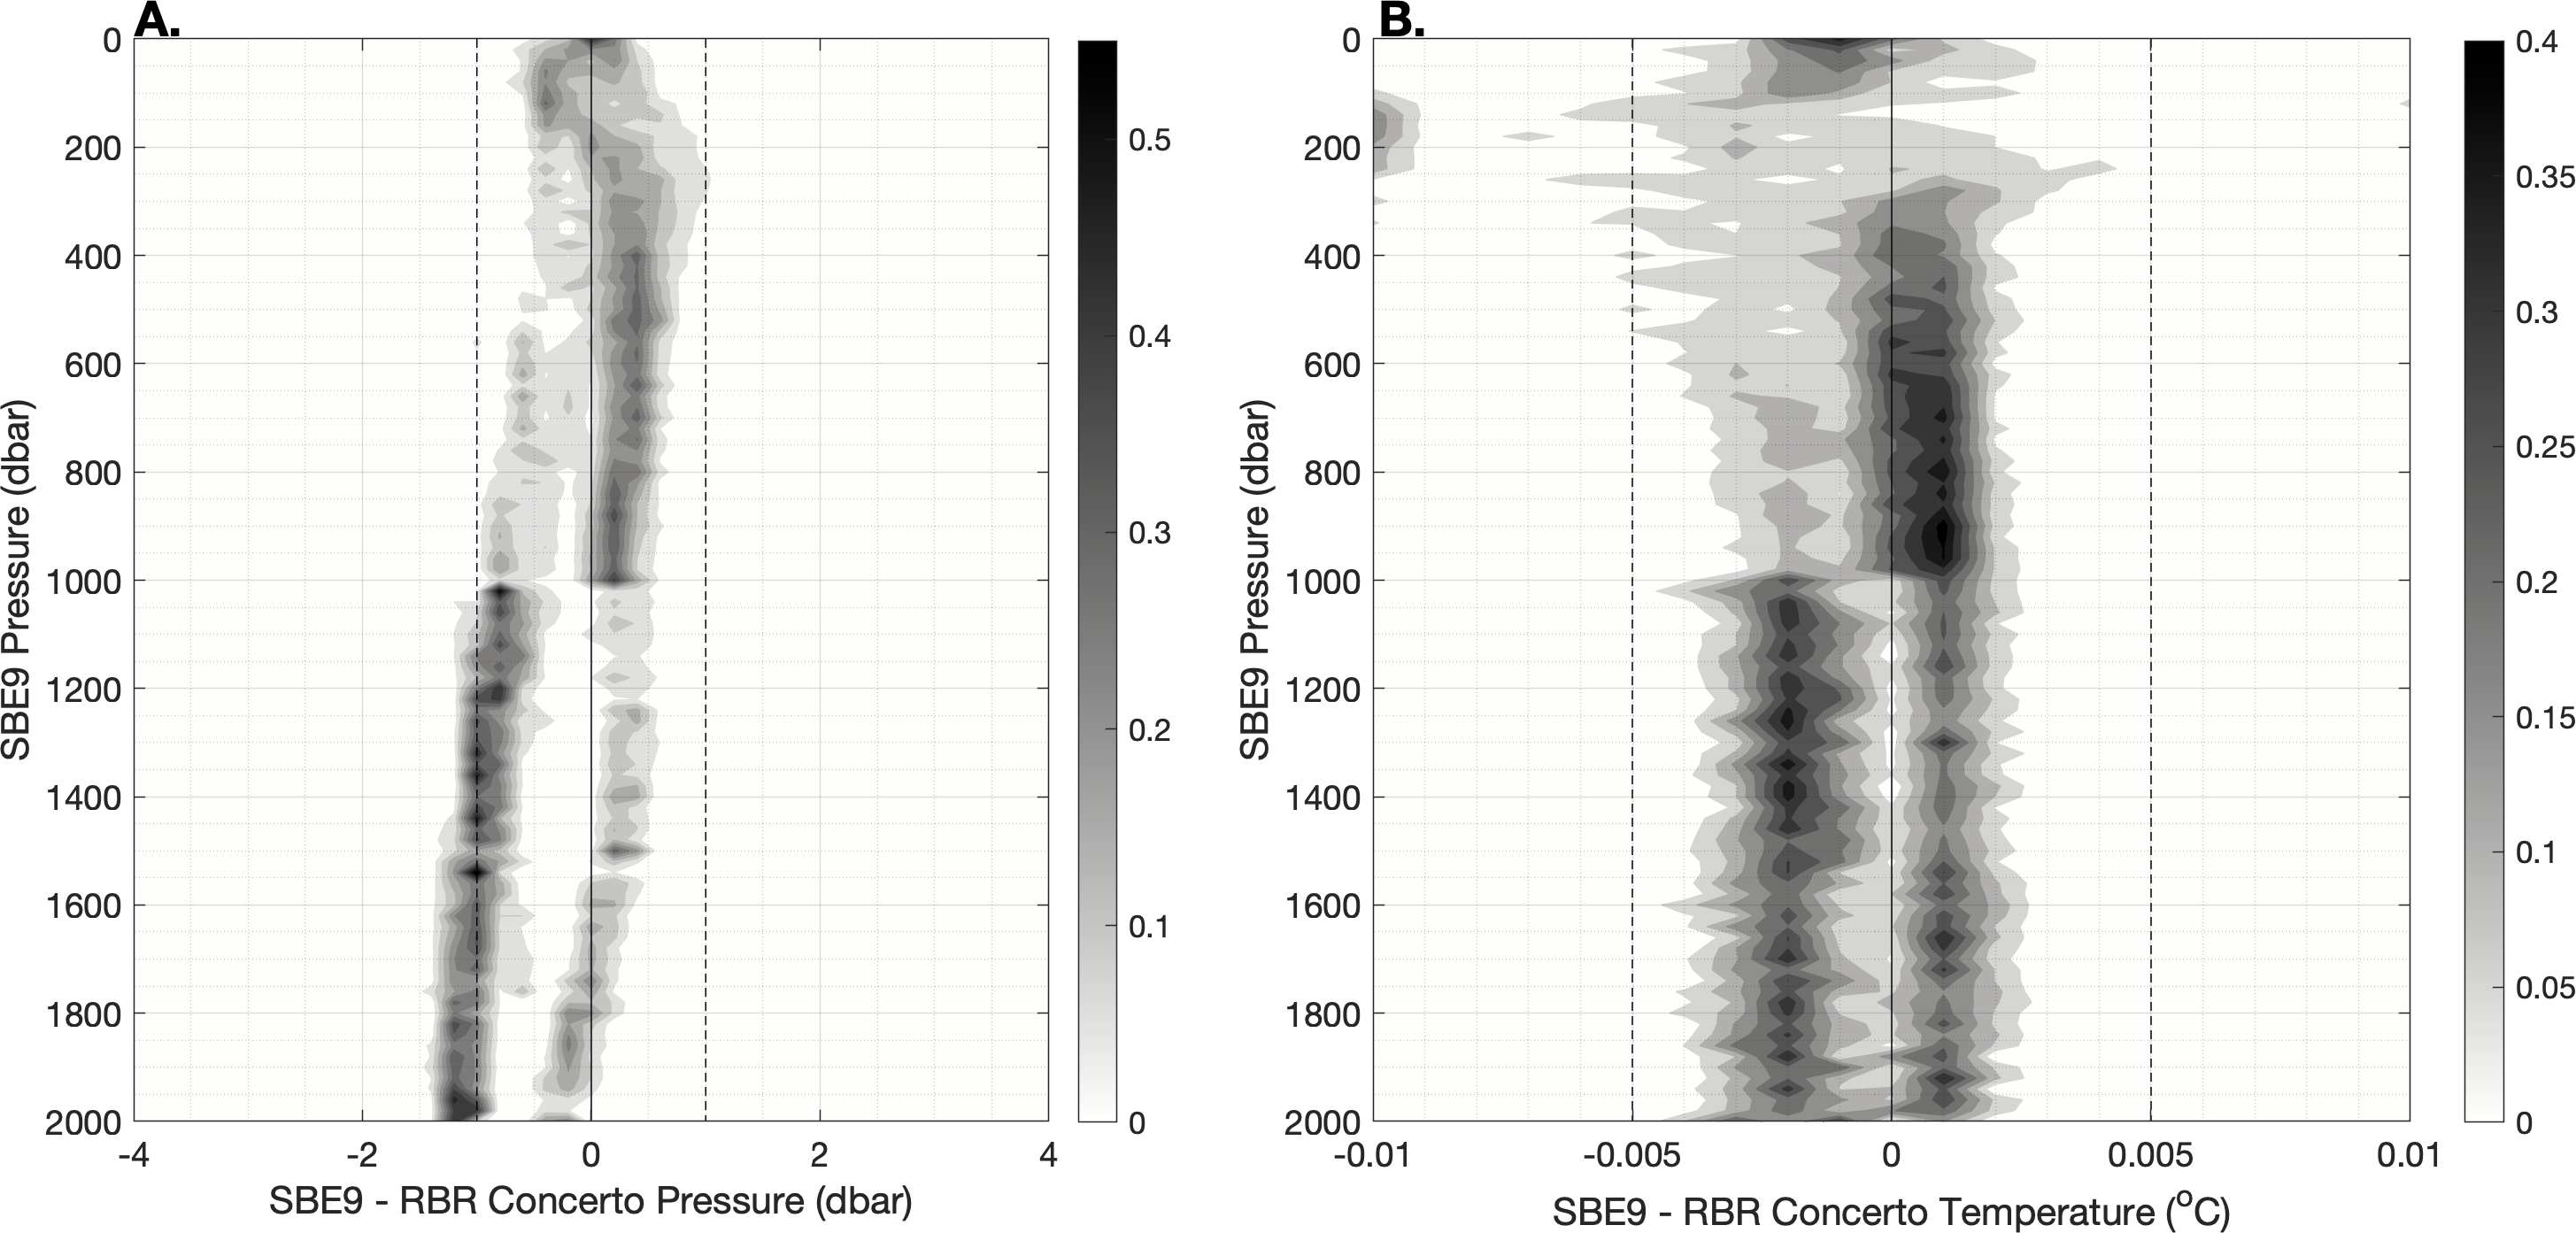
\includegraphics[width = \linewidth]{Fig3_PT_accuracy.png}\\
	\caption{(\textbf{A.}) Pressure differences between SBE9 and the RBR\textit{argo}$^3$ 's analogous RBR\textit{concerto}$^3$, across all voyages and sensor pairs, after synchronisation (see Section \ref{sec: static_datasets}).  Plotted is the frequency distribution in each 20 dbar SBE9 pressure bin, expressed as a fraction of the total pairs in 0.2 dbar increments of the difference.  (\textbf{B.}) Same as (\textbf{A.}) for temperature. Plotted is the frequency distribution in each 20 dbar SBE9 pressure bin, expressed as a fraction of the total pairs in 0.001 $^\circ$C increments of the difference. }
	\label{fig: PT_accuracy}
\end{figure}

A similar direct approach to examining temperature differences is precluded by the varying effect of water flow past the sensors within each rosette (the sensors are mounted at different heights above deck), and wake effects, which introduces both bias and noise to the comparison. 
To reduce these effects, we again use lagged correlations of the high-resolution temperature data streams from each sensor. 
For each cast and SBE9/RBR sensor pair, we perform a lagged correction of temperature tendency in each 15 dbar bin. 
For bins where the temperature tendency correlation coefficient is $>$ 0.5, we apply the lag, typically between 0-1 second) to align the temperature traces and then find the temperature differences. 
Thus for bins where wake effects de-correlate the temperature variance, the data are not used.  
As for pressure, the temperature differences are binned to produce frequency distributions in 20 dbar pressure bins (Figure \ref{fig: PT_accuracy}). 

Laboratory measurements are preferable to in-situ data for characterizing compressibility effects on the conductivity sensor.
For example, the natural variability in the upper layer of the ocean is larger than the target accuracy of the conductivity sensor ($\pm$ 0.003 mS/cm).
In a laboratory pressure tank data is collected for a range of pressures up to the maximum pressure rating (i.e., 2,000 dbar) of the RBR\textit{argo}$^3$.
The temperature of the pressure tank is maintained between 1 and 2 $^\circ$C to represent ocean conditions at depth. 
The salinity in the pressure tank is determined from water samples before and after the pressure cycling using a Guildline 8400B Autosal.

The effects of compressibility on the conductivity measurement can be modeled using a cubic adjustment of the form:
\begin{equation}
	C_{meas} = \frac{C_{raw}}{1 + X2\cdot P + X3\cdot P^2 + X4\cdot P^3}
	\label{eq: pressure_correction}
\end{equation}
where $C_{raw}$ is the raw conductivity measured by the instrument, $P$ is the sea pressure, ($X2$, $X3$, $X4$) is the set of compressibility correction coefficients, and $C_{meas}$ is the compressibility-corrected conductivity.

in-situ data from the YMC cruise in 2019 was used to validate the compressibility correction developed for two specific RBR\textit{argo}$^3$ CTDs (see Table \ref{tab: cruise_data}). 
A direct comparison can thus be made between the compressibility-corrected salinity collected from the RBR\textit{argo}$^3$ CTDs and the shipboard CTD, both cross-calibrated with water samples (see Appendix \ref{app: Kfactor}).

\subsection{Sensor stability}
A robust delayed-mode analysis method has been developed to identify salinity sensor drift in Argo profiling floats \citep{Owens_2009,  Cabanes_2016}. 
\cite{Nezlin_2020} used this method to characterize the long-term stability of the RBR\textit{argo}$^3$ on six early-deployed Argo floats.  
Here, we provide an update on the stability of the current RBR\textit{argo}$^3$ fleet, using nineteen RBR\textit{argo}$^3$ floats that have been sampling in the ocean for over six months. 
The time series of salinity from these nineteen RBR\textit{argo}$^3$ CTDs are compared against objectively mapped salinity from a CTD reference database. Comparisons are done on isotherms selected from the least variable part of the T-S curve in order to minimize the effects of natural variability in the comparison. 

\subsection{Dynamic behavior of conductivity measurements}
\label{sec: dynamic_datasets}
\subsubsection{Response time and sensor misalignments}
To align temperature and conductivity measurements collected by the RBR\textit{argo}$^3$, an optimal temporal lag is determined to correct the temperature observations. The optimal C-T lag, which combines the two mechanisms detailed in Section \ref{sec: theory}, is determined by maximizing the cross-correlation between the first-order differences in conductivity and in temperature \citep{Barth_1996,Ullman_2014,Dever_2020}. This approach relies on the assumption that changes in conductivity over short spatial scales are mostly driven by changes in temperature. The analysis is applied to data collected by six different RBR\textit{argo}$^3$ units deployed over different cruises (see Table \ref{tab: cruise_data}). Only downcasts sampling deeper than the mixed layer depth are used, as the RBR\textit{argo}$^3$ were pointing downwards in all deployments. The resulting dataset comprises a total of 380 profiles.
Each considered profile is separated into 7 s segments. 
For each segment, the cross-covariance between the first-order differences in temperature and in conductivity is computed for a series of lags. 
The lag maximizing the cross-covariance is recorded if the cross-covariance is greater than 0.5. 
Otherwise, the segment is rejected from the analysis, as it likely violates the fundamental assumption of this method. 
Segments located above the mixed layer depth are also ignored, as they would skew the results towards a maximum cross-covariance at a zero lag. 
A second-order polynomial is fit to the cross-covariance function using three consecutive points centred on the lag maximizing the cross-covariance. 
The polynomial's maximum determines the ``optimal lag" for the segment. 
Fitting a polynomial allows for non-integer lags, which is key to further remove dependence on the sampling rate. 
Finally, the optimal lags determined from all eligible segments are concatenated into a Probability Distribution Function (PDF) as a function of the profiling speed averaged over the length of the segment. 
A total of 25,488 segments are considered to determine the C-T lag for the thermistor on the RBR\textit{argo}$^3$. 
A Gaussian distribution is fit to the PDF in each profiling rate bin to extract the mean value of the C-T lag to be used to align temperature and conductivity readings.

\subsubsection{Thermal inertia errors}
An idealized experimental setup was designed in the laboratory to characterize how the RBR\textit{argo}$^3$ conductivity cell responds to thermal gradients. 
An RBR\textit{argo}$^3$ CTD was transferred from a cold bath (T$\approx$6$^\circ$C) into a large recirculating flume in thermal equilibrium with the room temperature (T$\approx$19$^\circ$C, S$\approx$30) to simulate a temperature step change in saltwater. 
The flume consists of a channel 50 cm wide by 50 cm high, and about 8 m long.  
At the upstream end of the channel, a collimator is used to smooth out the turbulence in the flow entering the channel.
At the downstream end of the channel, a propeller forces water through the recirculating loop at a constant speed, which can be adjusted by changing the rotational speed of the propeller. 
The water speed is monitored upstream of the RBR\textit{argo}$^3$ CTD by a current meter (Nortek Vector) with its sample volume centred on the same depth as the RBR\textit{argo}$^3$ CTD. 
Six different water speeds were configured between 7 and 45 cm/s, with two separate plunges at each speed. 

A correction for the long-term adjustment of the conductivity cell is computed using Equation \ref{eq: long-term_TM}.  
The coefficient ctcoeff is determined by doing a linear fit of the temperature anomaly as a function of the temperature difference between the interior of the conductivity cell and the water surrounding the cell.
For each plunge, data collected in the first 90 s are ignored to avoid contamination from the short-term thermal inertia adjustment. 
The temperature anomaly is then binned to avoid overweighting the fit towards low temperature gradients across the conductivity cell. 

The short-term error of the RBR\textit{argo}$^3$ conductivity cell responds to thermal gradients with a timescale on the order of seconds, and cannot be addressed using the same approach as for its long-term counterpart, mostly for practical reasons. 
The physical processes driving this short-term adjustment are hypothesized to be related to the exchange of heat between the water located within the cell's channel, and the ceramic itself. 
It is operationally challenging to directly measure the temperature of the ceramic. 
L\&P90 is used to correct the short-term thermal inertia on conductivity (see Equation \ref{eq: LP}).  
The timescale of the short-term thermal inertia adjustment is estimated first, using a similar approach to \cite{Lueck_1990b}: The slope of the logarithm of the normalized salinity time series is computed over the first 15 s after the temperature change to determine the e-folding timescale $\tau$, where $t = 0$ is defined as the time where the marine temperature reaches 99\% of its final value.
The optimal value of $\alpha$ is then computed by minimizing the root-mean-squared-error (RMSE) in the salinity residuals (Figure \ref{fig: short-term_TM}), referenced to the final static salinity. 

The results obtained from the flume are validated using in-situ datasets collected from two different profiling floats (see Table \ref{tab: float_data}). 
These specific floats were selected for several reasons: First, it is important that the data resolution is high enough to capture the relevant timescales. 
In fact, most profiling floats transmit data that are binned into pressure bins, thus smoothing out the relevant timescales and making the thermal inertia corrections inefficient, especially over the shorter timescales. 
Second, it is necessary to have well-defined,  sharp, interfaces followed by a well-mixed layer to be able to visualize the salinity adjustment due to thermal inertia. 
This is often the case in either thermohaline staircases, or at the base of the surface mixed layer. 
Finally, these floats were selected because they span different ocean basins (Caribbean Sea and sub-arctic North-Atlantic), and a range of profiling speeds ranging from 3 cm/s to 20 cm/s.


\section{Results}
\label{sec: results}
\subsection{Static accuracy and compressibility correction}

\subsubsection{Pressure and Temperature accuracy}
Figure \ref{fig: PT_accuracy} demonstrates the static accuracy of both pressure and temperature on the RBR\textit{argo}$^3$ when compared to a SBE9 on a CTD rosette.  The full data set reveals that the instruments agree to within 1.5 dbar across all pressure ranges.  For temperature, we find that the vast majority of paired readings give temperature differences less than 0.003$^\circ$C, which is within the specifications of the SBE9 and RBR\textit{argo}$^3$ CTDs, confirming the stated accuracy for temperature on the RBR\textit{argo}$^3$  across the pressure ranges examined.

\subsubsection{Conductivity static accuracy}
\label{sec: static_results}
The amplitude of the compressibility error was characterized by directly comparing the salinity profiles obtained from an SBE9 and RBR\textit{argo}$^3$ CTDs on a variety of cruises.  
Comparing the two salinity records in the deeper part of the water column (e.g.,  $>$800 dbar),  where the water masses tend to be more stable,  revealed that the salinity difference between the RBR\textit{argo}$^3$ CTDs and the shipboard cross-calibrated SBE9 has a depth-dependent bias.  
An example of this bias is showed in Figure \ref{fig: YMC_data} using the data from the YMC cruise (see Table \ref{tab: cruise_data}).  
Both RBR\textit{argo}$^3$ CTDs tested on the YMC cruise have a salty bias that increases with depth,  suggesting that the error in salinity is caused by the compressibility of the conductivity cell. 

\begin{figure}[t]
	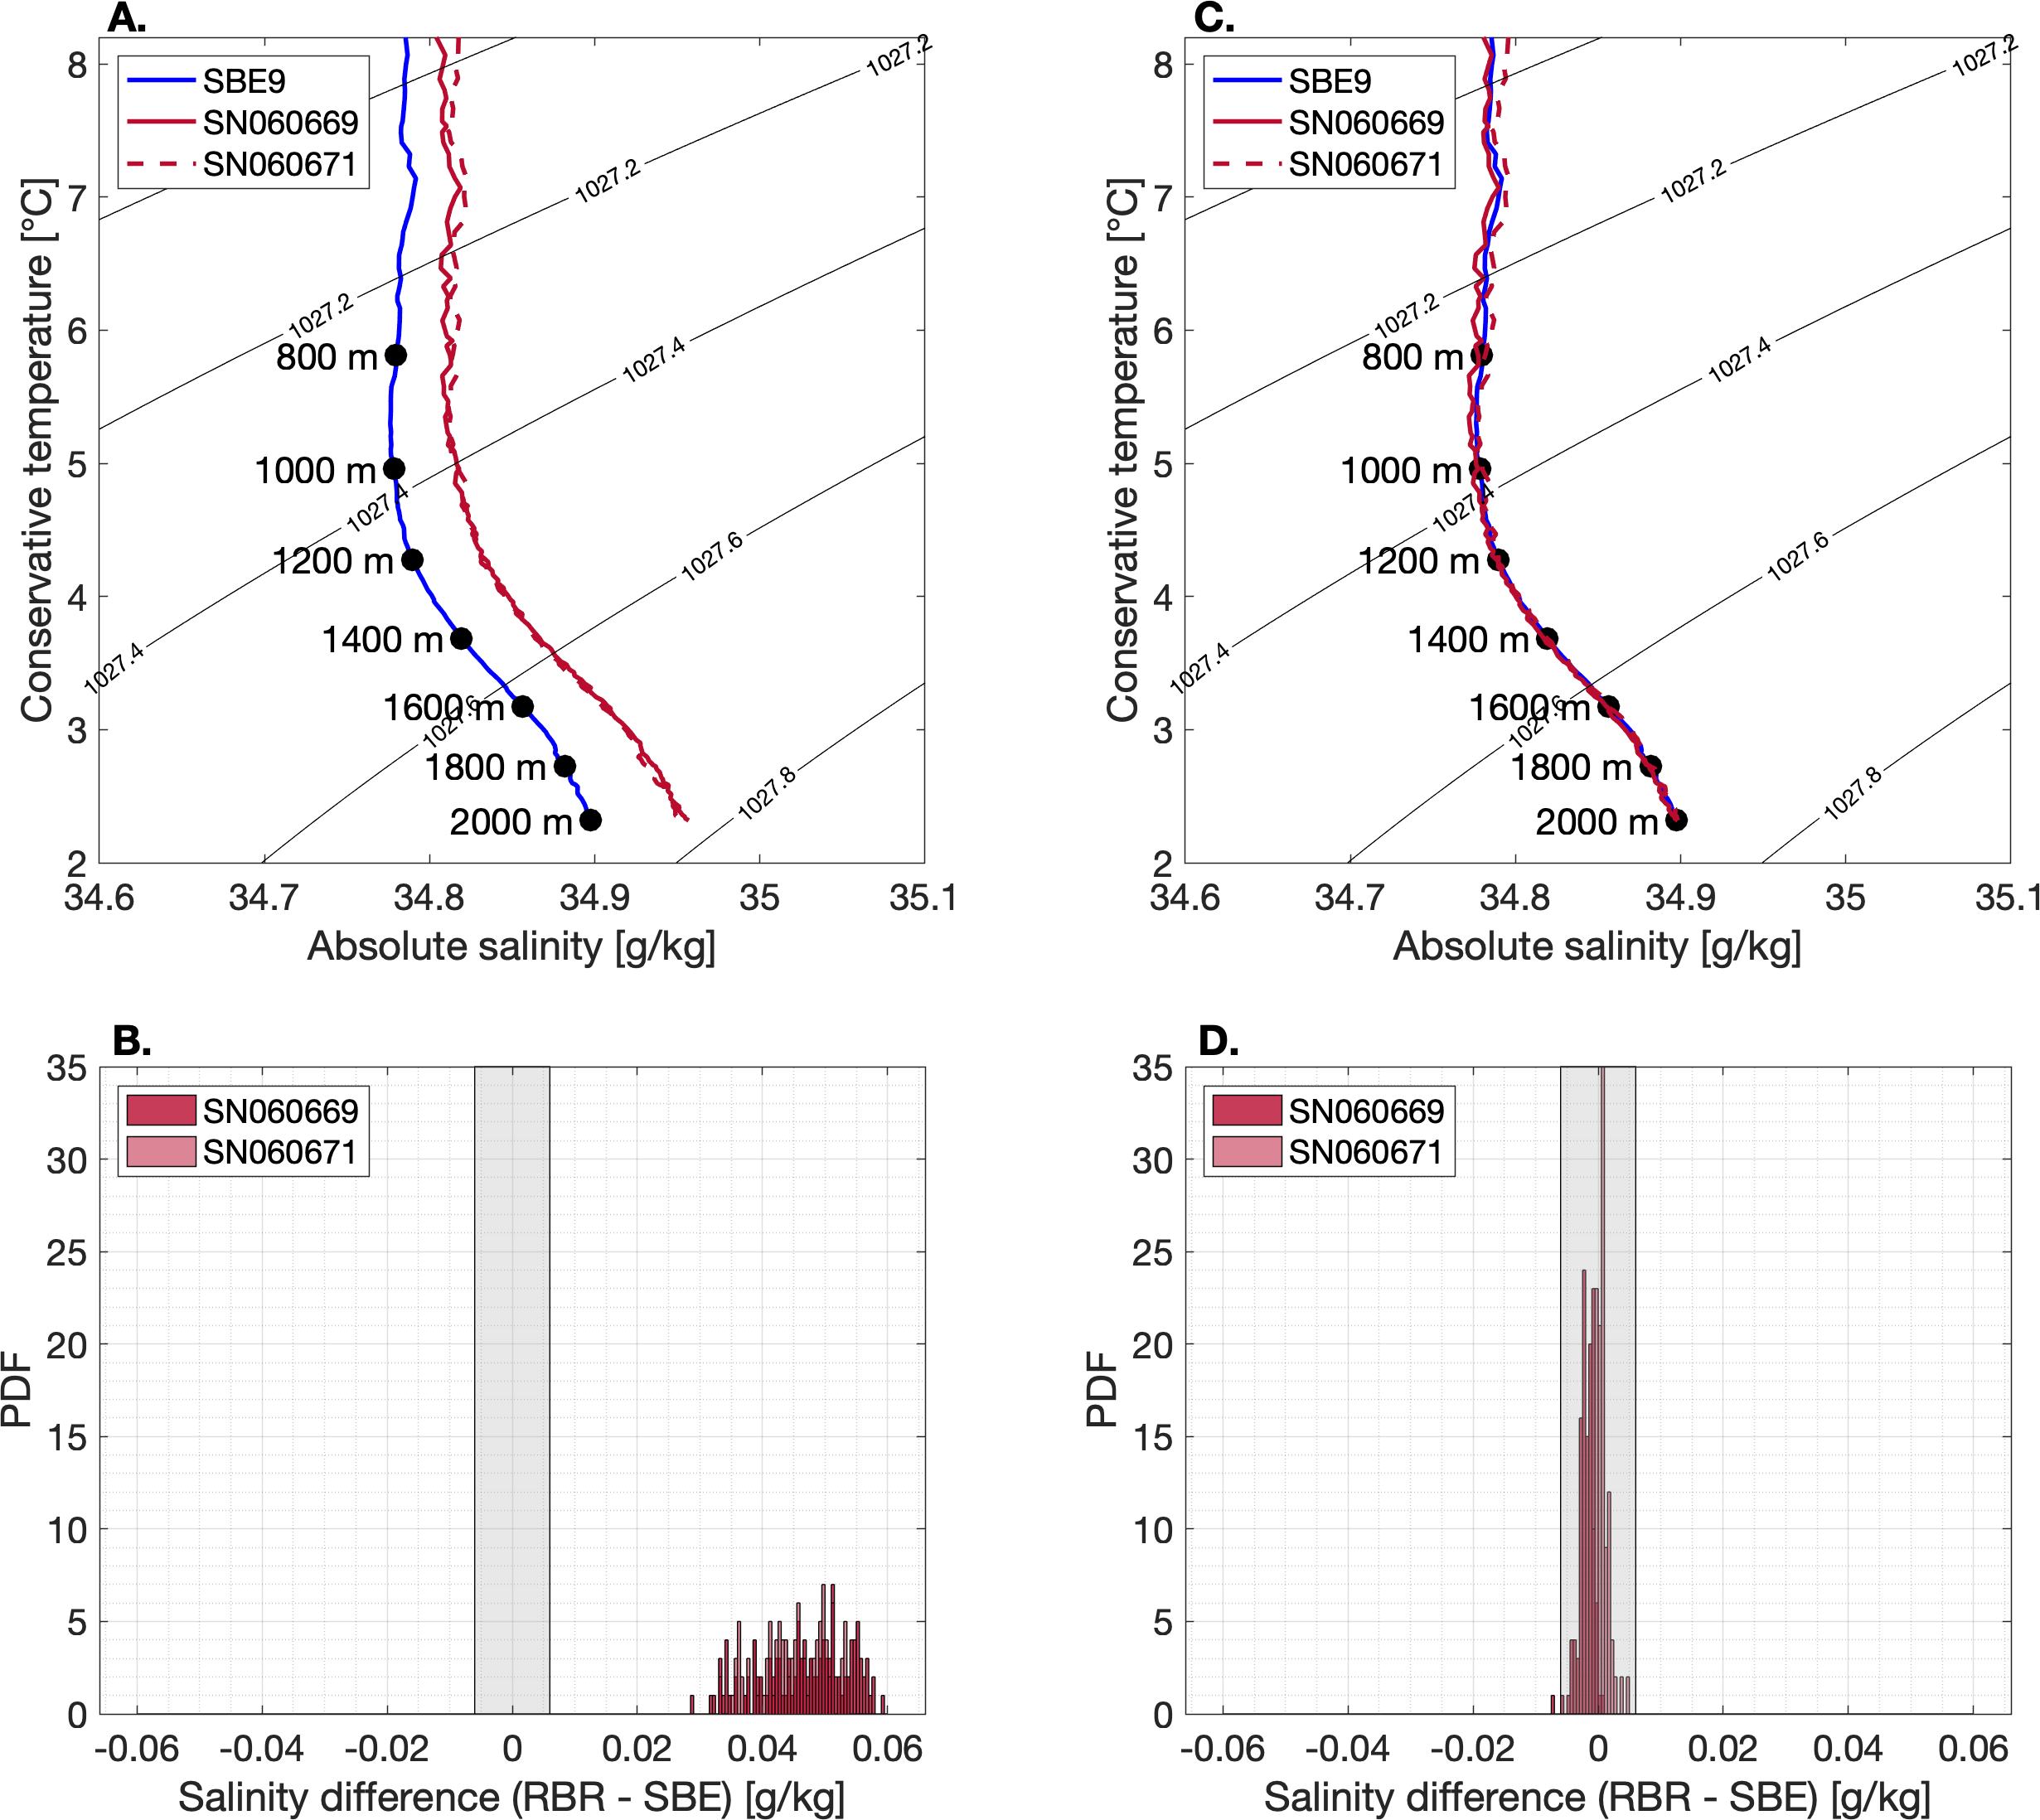
\includegraphics[width = \linewidth]{Fig4_compression_errors_YMC.png}\\
	\caption{T-S plots of data collected by two RBR\textit{argo}$^3$ and a SBE9 during the YMC cruise \citep[station 4; ][]{YMCreport_2019} (\textbf{A.}) before and (\textbf{C.}) after applying a customized pressure correction to conductivity. The corresponding Probability Distribution Functions (PDFs) of the salinity bias for data collected below 800 m are shown in (\textbf{B.}) and (\textbf{D.}).  All three CTDs were cross-calibrated using bottle samples taken on this profile (see Section \ref{sec: theory} and Appendix \ref{app: Kfactor}).}
	\label{fig: YMC_data}
\end{figure}

The two RBR\textit{argo}$^3$ CTDs deployed on the YMC cruise were subsequently tested for pressure response in the laboratory,  using the setup described in Section \ref{sec: static_datasets}.  
Customized coefficients were derived for each RBR\textit{argo}$^3$ CTD,  reducing the compressibility-induced salinity error from O(0.02)  to $<$0.003  (Figure \ref{fig: saltbladder_results}).  
The field-based comparison confirms the validity of the newly-derived compressibility correction coefficients from the laboratory: after updating the coefficients in Equation \ref{eq: pressure_correction},  both RBR\textit{argo}$^3$ CTD compare well to the calibrated SBE9 data,  with residuals contained within the combined accuracies of the RBR\textit{argo}$^3$ and the SBE9 CTDs (Figure \ref{fig: YMC_data}).  
Not only the mean of the PDF is brought closer to 0,  its standard deviation is also reduced,  suggesting that the salinity bias is less dependent on depth. These results indicate that customized parameters for compressibility correction to conductivity can reliably be determined for individual RBR\textit{argo}$^3$ CTDs in the laboratory during the calibration process.

\begin{figure}[t]
	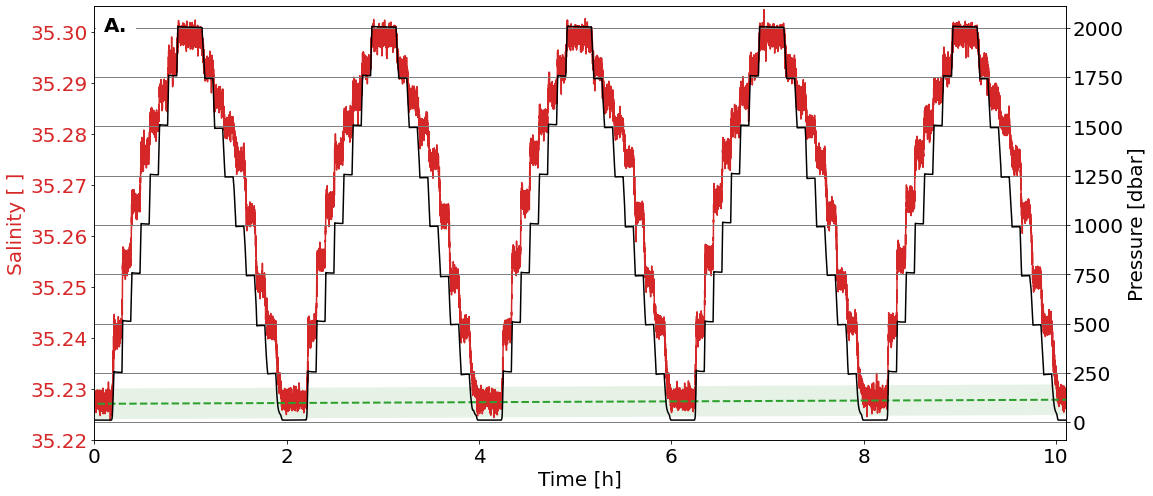
\includegraphics[width = \linewidth]{Fig5_Pressure_correction_raw}\\
	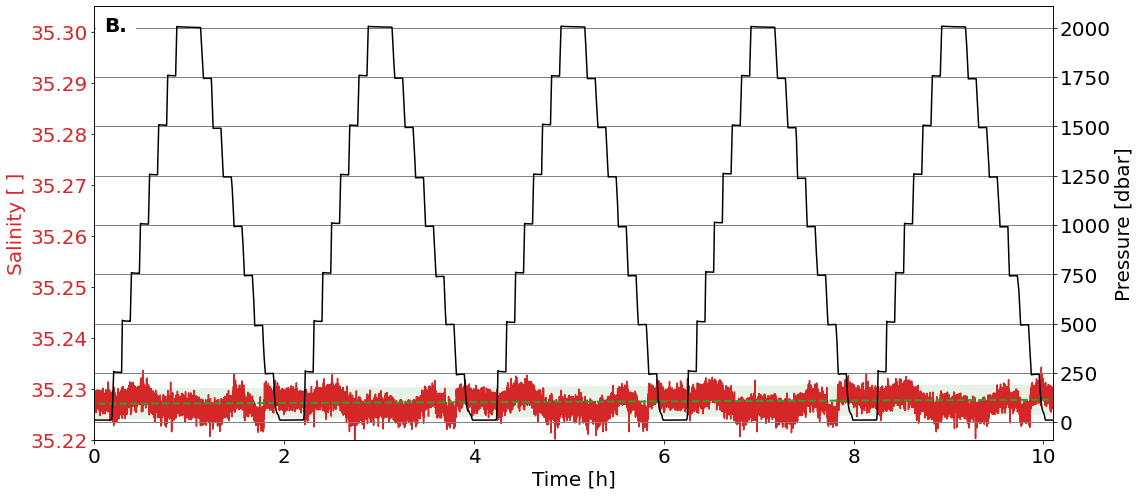
\includegraphics[width = \linewidth]{Fig5_Pressure_correction_corr}\\
	\caption{Time series of practical salinity (red line) during pressure cycling (black line). (\textbf{A.}) before pressure correction is applied, and (\textbf{B.}) after the cubic pressure correction has been applied for the RBR\textit{argo}$^3$ CTD SN060671.  The reference salinity is super-imposed (dashed green line), with its associated uncertainties (green shading).}
	\label{fig: saltbladder_results}
\end{figure}

\subsection{Sensor stability}
Since the average length of the time series from the nineteen considered RBR\textit{argo}$^3$ CTDs was only 1.5 years, it is somewhat premature to draw any definite conclusions about the long-term stability of the RBR\textit{argo}$^3$ CTDs. 
Nonetheless, salinity measurements from eighteen RBR\textit{argo}$^3$ CTDs showed no sign of sensor drift at the time of analysis, suggesting good sensor stability (Figure \ref{fig: stability}). 
Only one RBR\textit{argo}$^3$ suffered from significant drifting (WMO5906299), which was identified to be associated with a malfunction of the float's buoyancy pump. 
The float was found to have extended surfacing times, sometimes over 24 hours,  that correlated with sudden and large fresh salinity errors, suggesting the cell suffered from biofouling due to the abnormally long surfacing time \citep{RBRdrift}.
For the remaining eighteen RBR\textit{argo}$^3$ CTDs,  totalling 857 profiles to date, 94\% of profiles have a salinity anomaly smaller than $\pm$0.01 , falling within Argo's expectation.  
As in Section \ref{sec: static_results}, an offset from reference was present for most of the analyzed CTDs, which is due to the sub-optimal compressibility coefficients used on these RBR\textit{argo}$^3$ CTDs, as previously discussed.

\begin{figure}[t]
	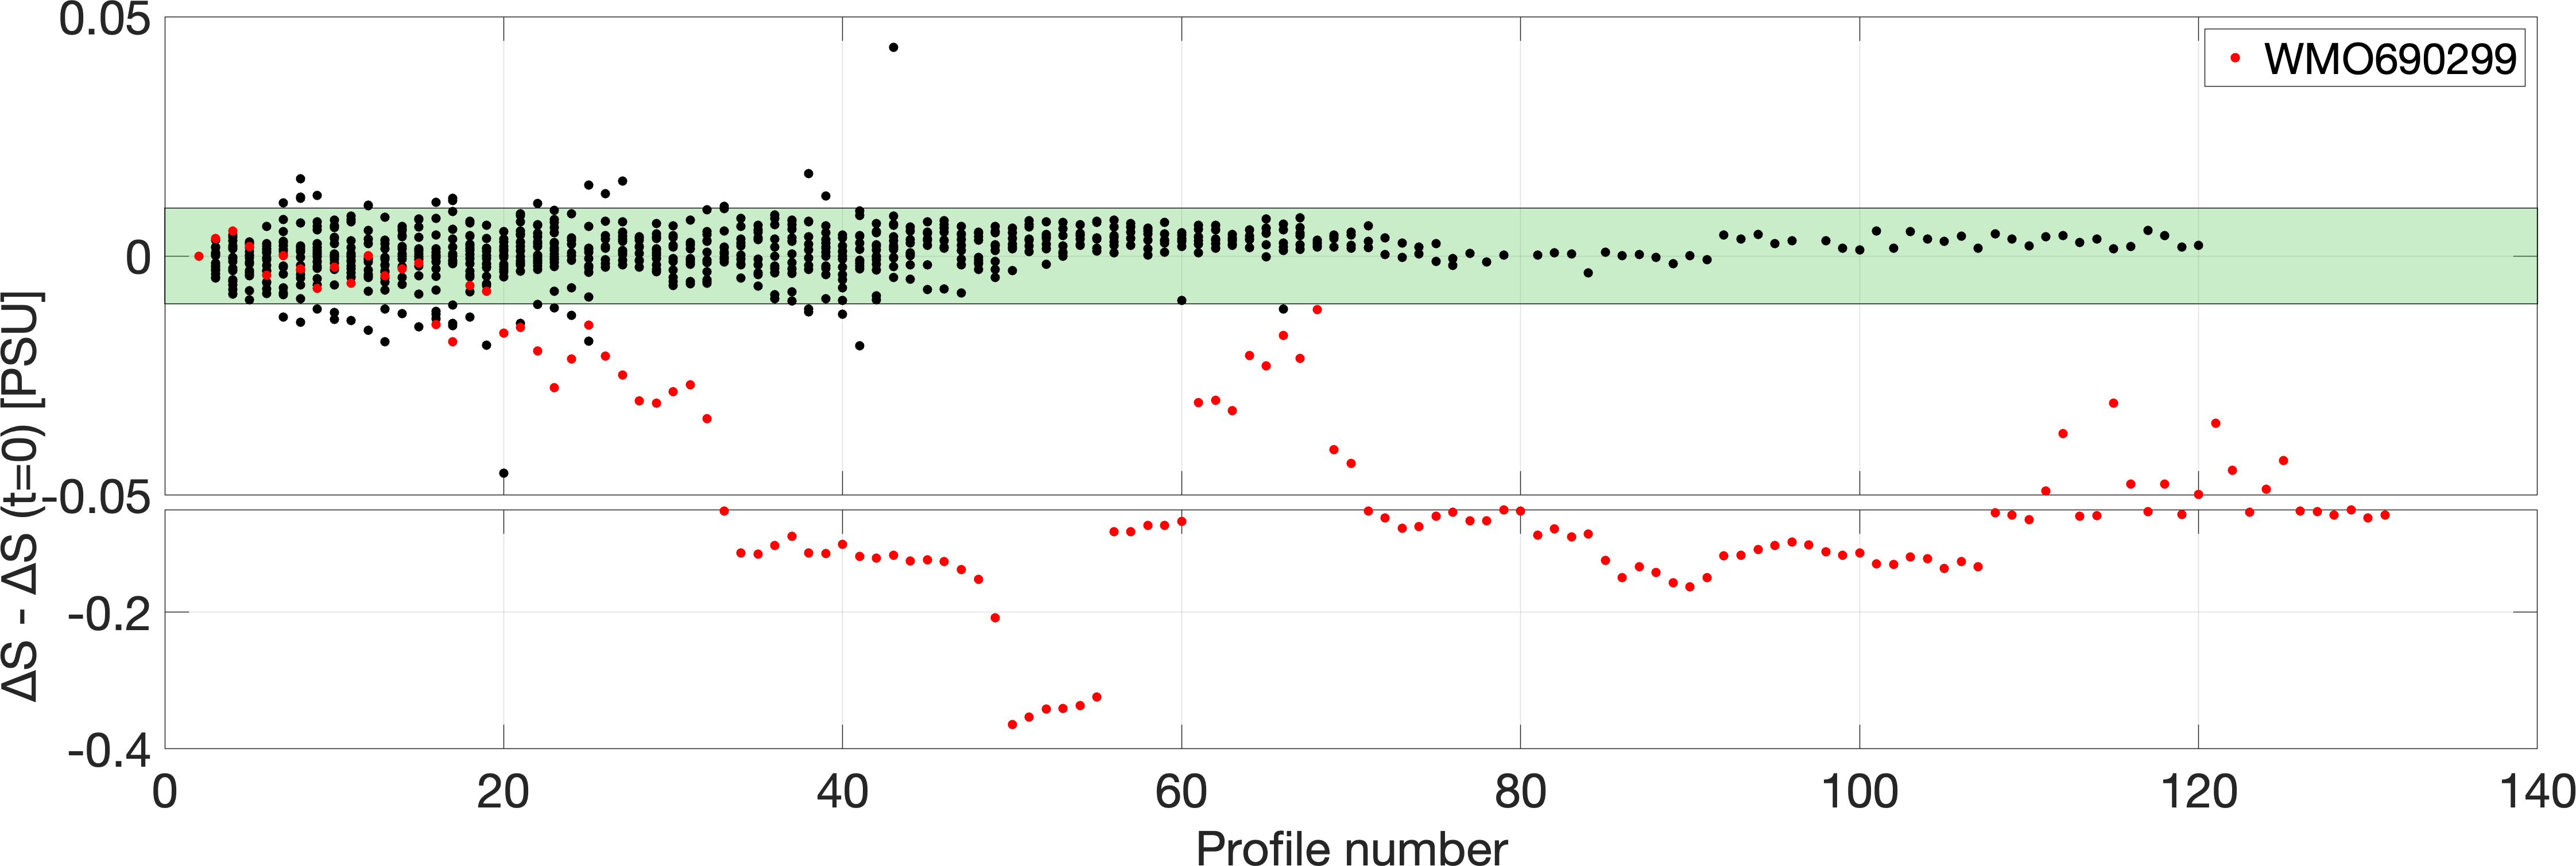
\includegraphics[width = \linewidth]{Fig6_stability}\\
	\caption{Time series of the salinity bias determined from objectively mapped reference data \citep{Owens_2009} with respect to the first full-depth profile,  for nineteen RBR\textit{argo}$^3$ CTDs. The green shading indicates +/- 0.01 . Float with WMO5906299 is highlighted in red, as it was identified to drift due to a float malfunction (see Section \ref{sec: results}). Note the break and change in scale in the y-axis.}
	\label{fig: stability}
\end{figure}


\subsection{Dynamic behavior of conductivity measurements}
\subsubsection{Response time and sensor misalignments}
The misalignment between temperature and conductivity measurements (i.e., C-T lag) introduced by the slower time-response of the thermistor is characterized by applying the analysis detailed in Section \ref{sec: datasets}.  The distribution of ``optimal" C-T lags derived from the dataset is shown in Figure \ref{fig: CT_lag}.  Several key points can be extracted from Figure \ref{fig: CT_lag}: First,  the spread between the 25$^{th}$ and 75$^{th}$ percentiles with respect to the median value is comparable across fall-rates,  suggesting that the distribution of optimal lags can be approximated by a normal distribution.  Second,  the median value computed for each individual fall-rate bin is fairly constant and thus does not seem to be a function of the fall-rate,  over the range of rates explored.  Third,  a constant optimal lag of 0.350 s ($\sigma$= 0.003 s) can be used for fall-rates slower than 1.5 dbar/s.

\begin{figure}[t]
	\centering
	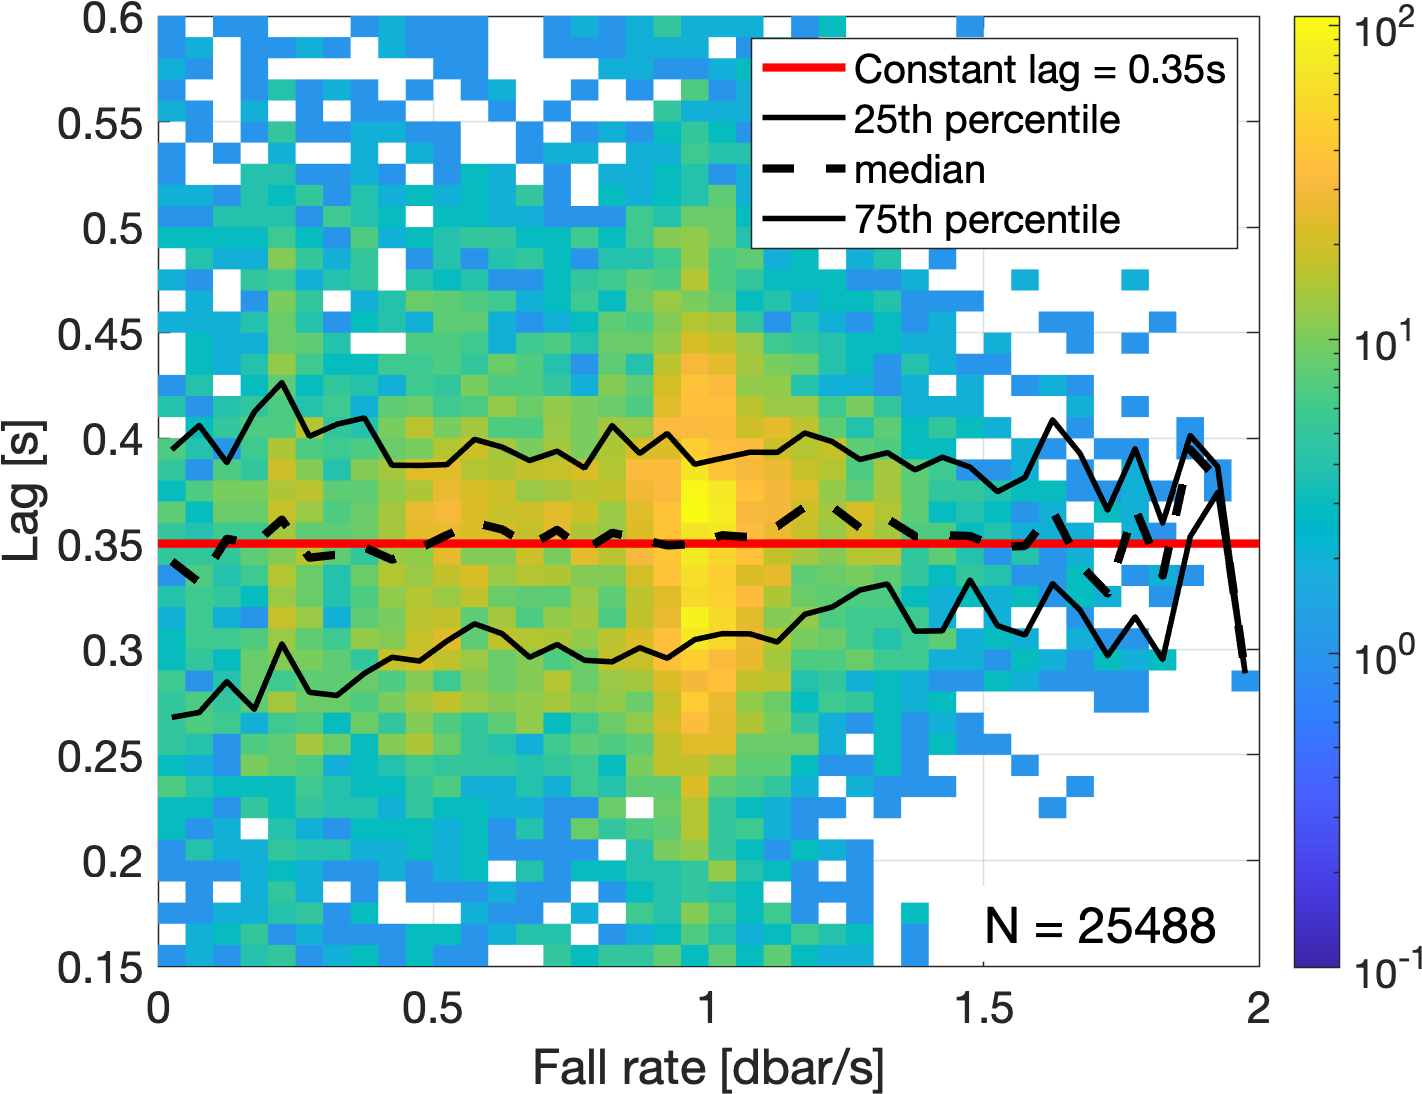
\includegraphics[width=.7\linewidth]{Fig7_RBRargo_CTlag_2DPDF}
\caption{Two-dimensional PDF of the ``optimal" C-T lag derived for 25,488 segments,  as a function of fall-rate (see Section \ref{sec: datasets}).  Note the logarithmic color scale.}
	\label{fig: CT_lag}
\end{figure}

To validate this empirically-derived C-T lag with an independent dataset, an RBR\textit{argo}$^3$ CTD is used in the laboratory to profile downward through a sharp temperature gradient \citep[Figure \ref{fig: WHOI_tank}; ][]{Schmitt_2005}.  It is clear in Figure \ref{fig: WHOI_tank} that the time-response of the temperature lags the response of the conductivity measurements: Not only the interface is smoother in the temperature signal than it is in the conductivity measurements, it is also shifted in time (and thus pressure).  The computed salinity exhibits a spike just after the RBR\textit{argo}$^3$ CTD crossed the interface, with a maximum error of 1.5 . Once the C-T lag correction is applied, the interfaces in both temperature and conductivity are centred around $\sim$ 3 dbar. Spiking observed in the raw salinity is now much reduced and the bottom layer is more homogeneous.  

\begin{figure}[t]
	\centering
	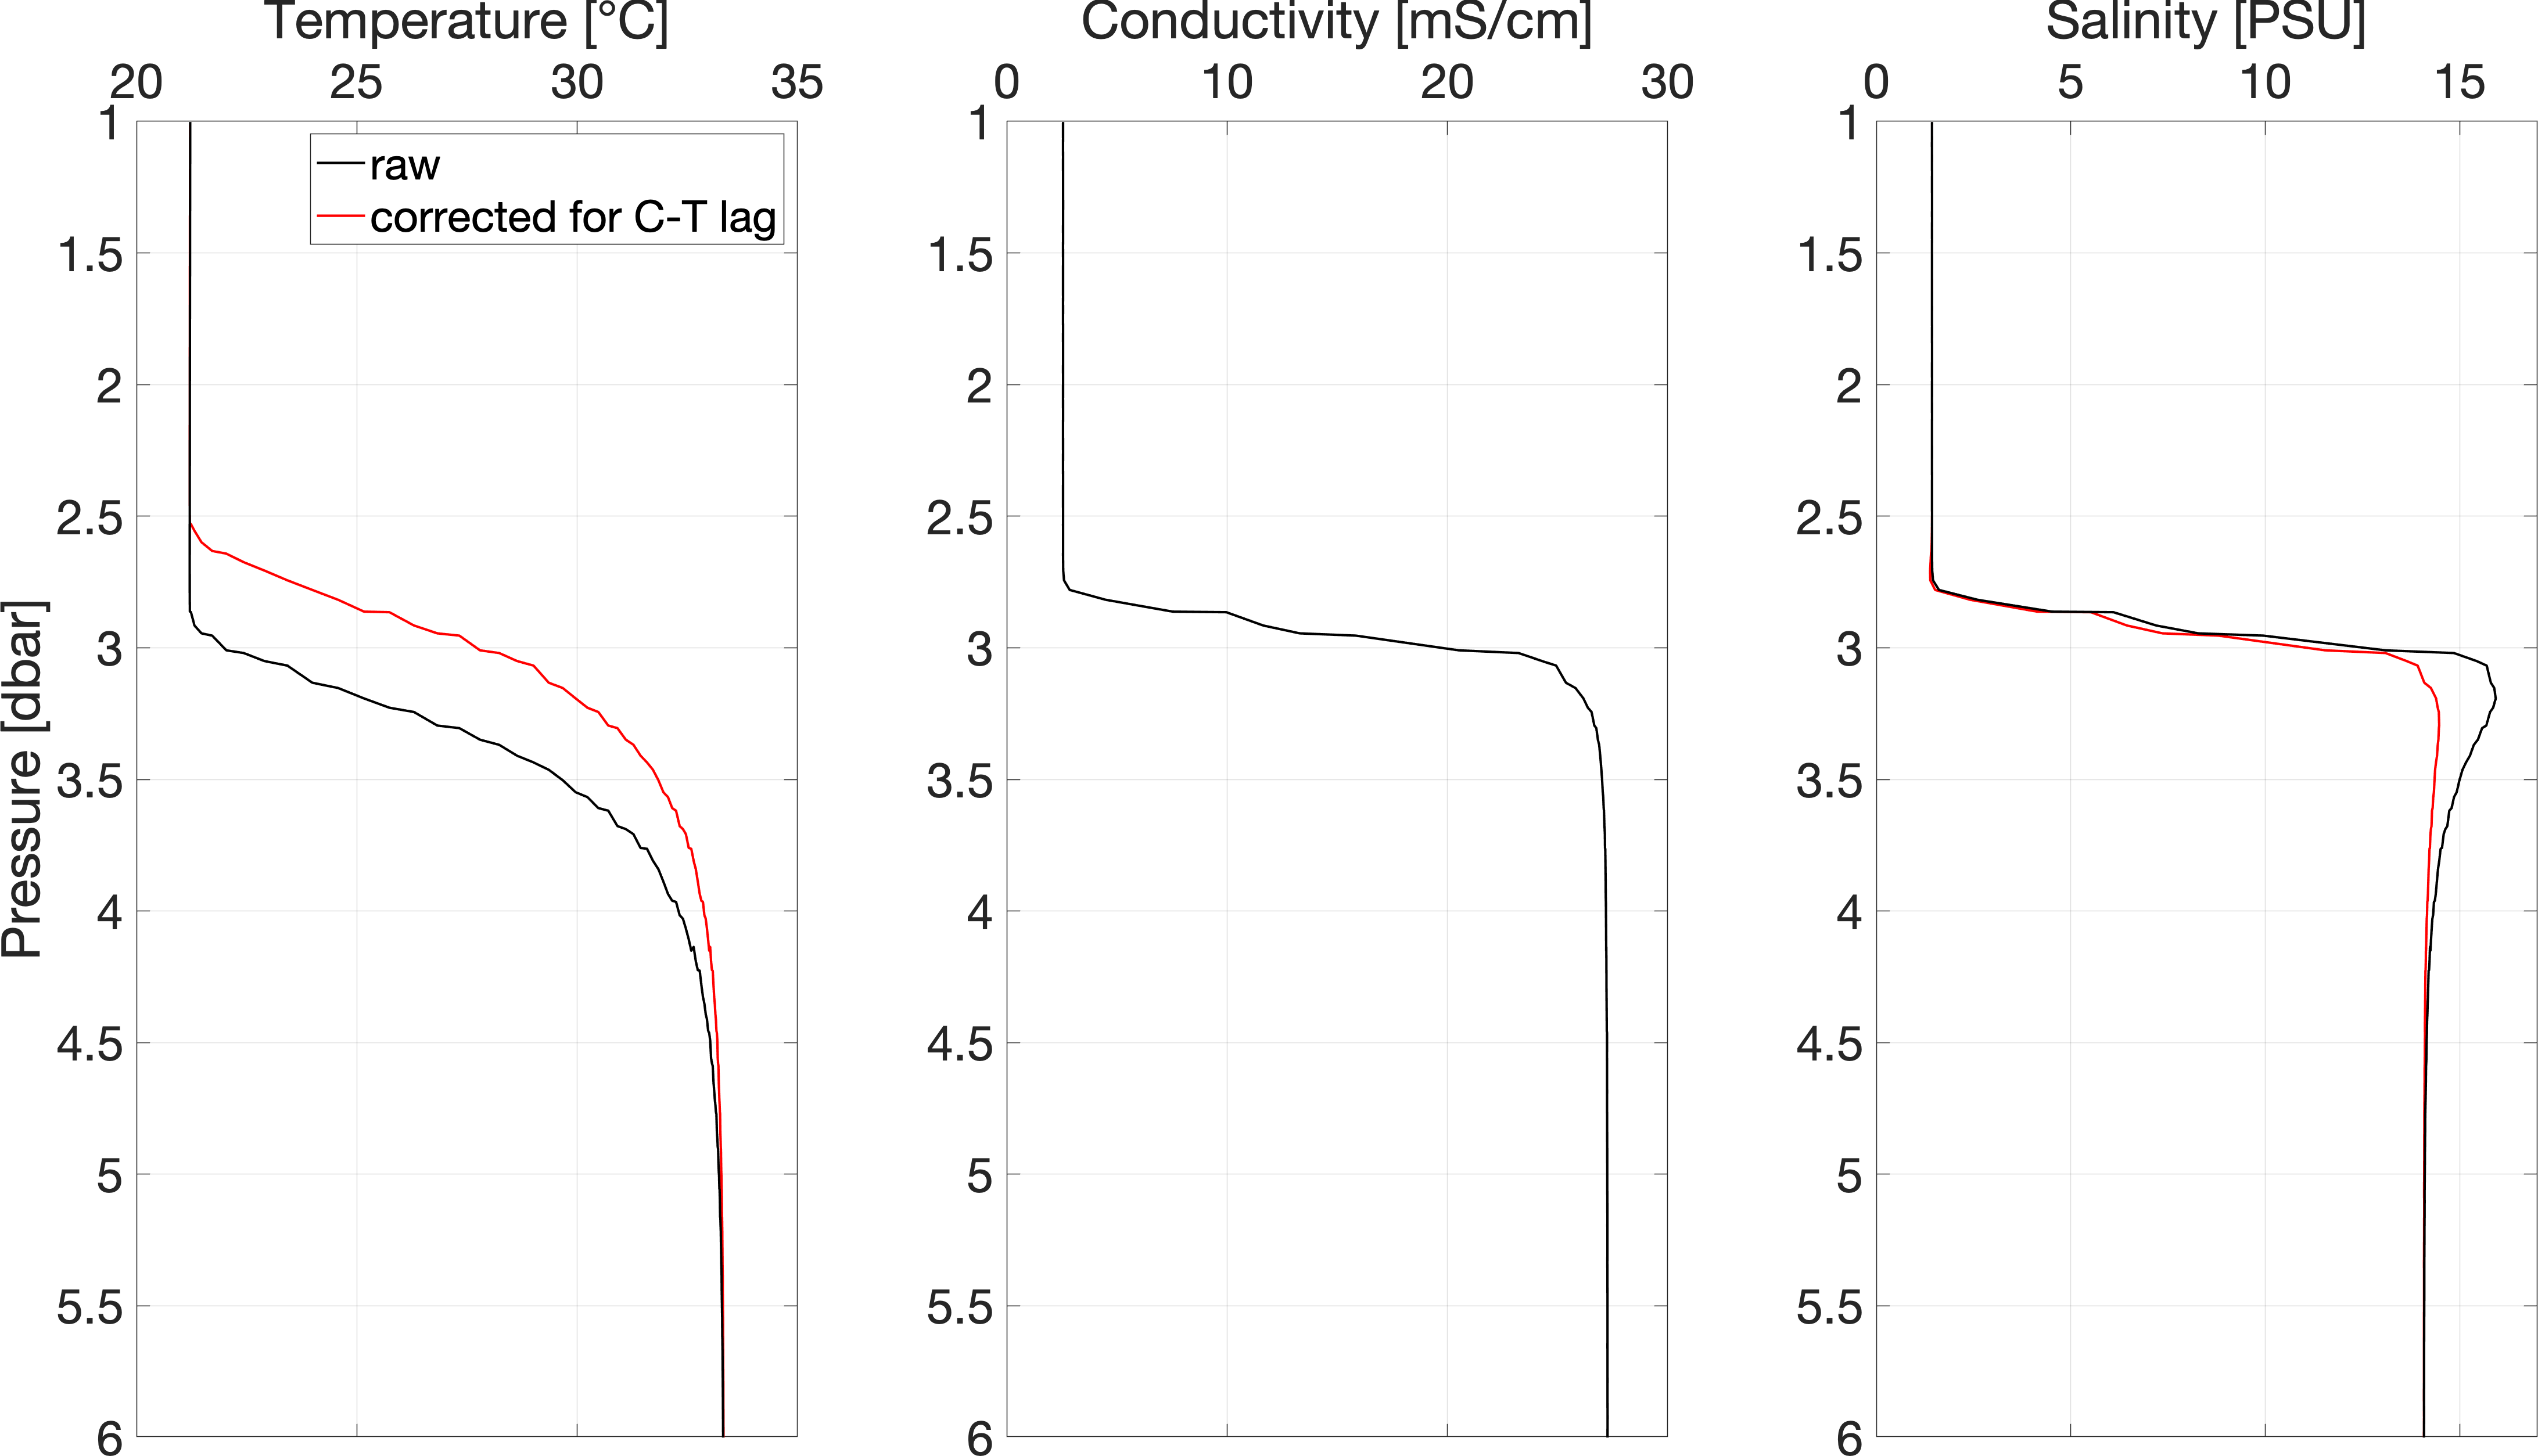
\includegraphics[width=.9\linewidth]{Fig8_Profile_example_CTlag}
	\caption{Profiles of temperature, conductivity, and salinity obtained using an RBR\textit{argo}$^3$ across a sharp temperature and conductivity interface in a water tank \citep{Schmitt_2005}. Lagging the temperature signal in time by -0.35 s reduces salinity spiking seen at the interface.}
	\label{fig: WHOI_tank}
\end{figure}

\subsubsection{Thermal inertia errors}
Figure \ref{fig: long-term_TM} shows the two dominant timescales of the thermal inertia adjustment of the salinity after experiencing a temperature change, and highlights the change in physical processes responsible for those two different timescales. 
At first, the salinity error normalized by the temperature change, is as large as 0.02 1/$^\circ$C and rapidly adjusts with a characteristic timescale on the order of tens of seconds. During this first phase, the temperature difference between the water and the internal cell temperature does not constitute a good predictor, suggesting that the driving mechanism is the heat exchange between the ceramic and the sampled water volume, as hypothesized in Section \ref{sec: datasets}.
For longer timescales ($>$30 s), the temperature gradient across the conductivity cell $\Delta$T becomes a good predictor of the thermal inertia temperature anomaly. As $\Delta$T decreases and the conductivity cell reaches thermal equilibrium with its surrounding water, the corresponding temperature anomaly decreases linearly with a constant slope.
Once the long-term correction is applied using Equation \ref{eq: long-term_TM}, the transient salinity error depicted in Figure \ref{fig: long-term_TM} is greatly reduced. The remaining thermal inertia error is now mostly constrained to the first tens of seconds after the temperature step. For example, at $V_p$ = 13.2 cm/s,  the salinity error after 60 s drops from 5$\times$10$^{-3}$ to 5$\times$10$^{-4}$ 1/$^\circ$C.

\begin{figure}[t]
	\centering
	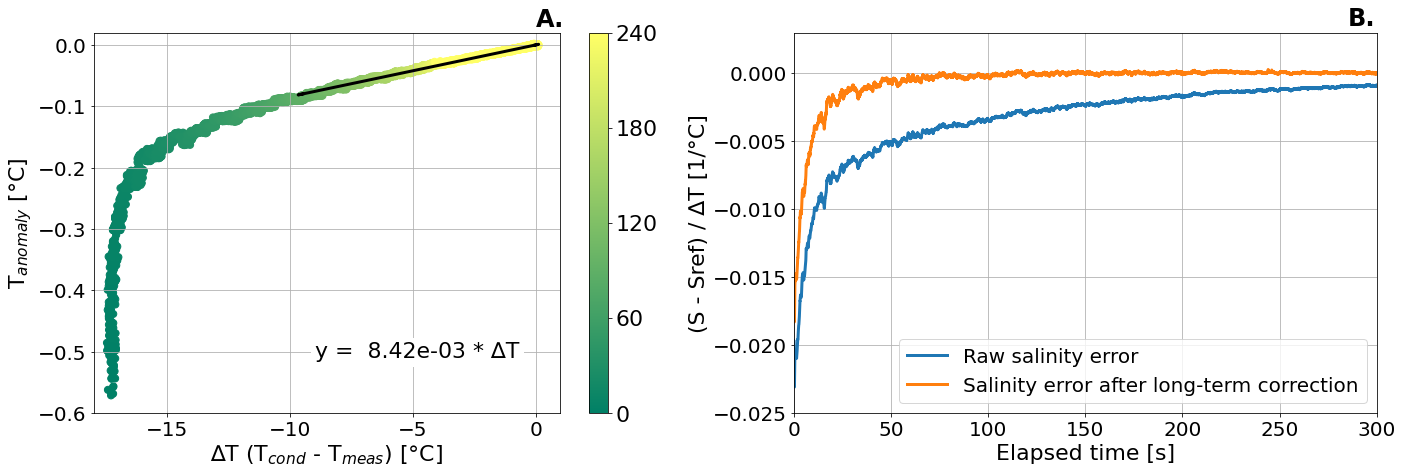
\includegraphics[width=\linewidth]{Fig9_long_term_TM} \quad
	\caption{Example of long-term correction for SN208077 at a flow speed of 13.2 cm/s. (\textbf{A.}) Computed temperature anomaly $T_{anomaly}$ as a function of the temperature difference between T$_{cond}$ and T$_{meas}$ (see Section \ref{sec: static_datasets}). Colormap shows the time elapsed since the temperature step-change in seconds, and the solid black line shows the least-squares fit used to compute $\text{ctcoeff}$. (\textbf{B.}) Time series of salinity error during the plunging test, normalized to the temperature gradient (see Section \ref{sec: plunging}).  Raw salinity (blue) is shown along with the corrected salinity (orange) using Equation \ref{eq: long-term_TM} and $\text{ctcoeff} = 8.42\times10^{-3}$. }
	\label{fig: long-term_TM}
\end{figure}


The remaining error in the salinity is attributed to the thermal inertia adjustment over short timescales.  This adjustment over shorter timescales can be seen in the time series of the normalized salinity in Figure \ref{fig: short-term_TM}, where the logarithm of the normalized salinity decreases linearly with time. 
A linear fit over the first 15 s after the temperature step yields an estimate of the e-folding timescale $\tau$. For example, at $V_p$ = 13.2 cm/s, the normalized salinity decreases with a time constant of $\tau$ = 8.0 s.  Using this decaying timescale,  it is found that $\alpha$ = 0.03 minimizes the RMSE of the salinity residuals. 
Figure \ref{fig: short-term_TM} shows the time series of salinity residuals after correcting for both the long- and short-term thermal inertia errors for $V_p$ = 13.2 cm/s, with a maximum salinity residual on the order of 1 $\times$10$^{-3}$ 1/$^\circ$C.

\begin{figure}[t]
	\centering
	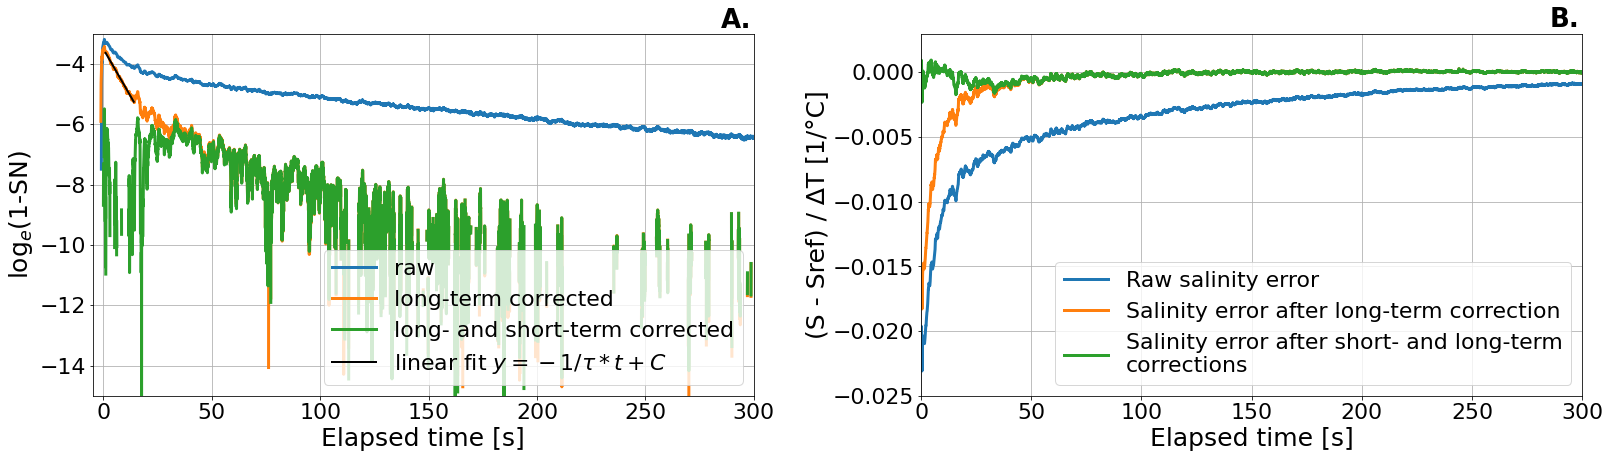
\includegraphics[width=\linewidth]{Fig10_short_term_TM}
	\caption{Example of short-term correction for SN208077 at a flow speed of 13.2 cm/s. (\textbf{A.}) Time series of the normalized salinity error. The linear fit used to derive the timescale $\tau$ (see Section \ref{sec: plunging} and Equation \ref{eq: LP2}) is shown as the solid black line. (\textbf{B.}) Time Series of the salinity error during the plunging test normalized to the temperature gradient, similarly to Figure \ref{fig: long-term_TM}.}
	\label{fig: short-term_TM}
\end{figure}

All three coefficients used in correcting for thermal inertia errors are expected to vary with the profiling speed $V_p$, as the profiling speed affects the thickness of the boundary layer around the conductivity cell, in turn changing the magnitude and timescale of the heat fluxes\citep{Lueck_1990a, Morison_1994}. 
Figure \ref{fig: TM_vs_speed} shows how each of the coefficients vary with the flow speed. 
All three coefficients can be fit to a power-law:

\begin{figure}[t]
	\centering
	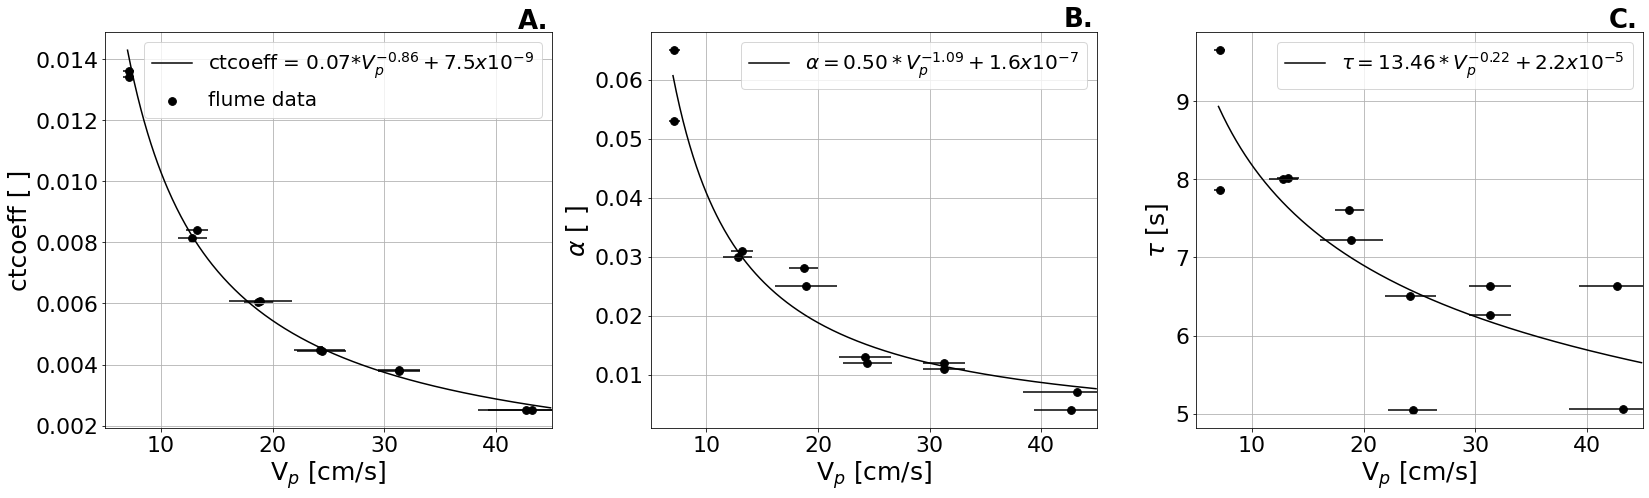
\includegraphics[width=\linewidth]{Fig11_TM_vs_speed}
	\caption{Values of the measured ctcoeff, $\alpha$, and $\tau$ as a function of the flume speed V$_p$ (black circles). The standard deviation in the water speed measured during each plunge is shown as error bars. A power-law least-squares fit is applied to the data (dashed black line).}
	\label{fig: TM_vs_speed}
\end{figure}


\begin{align*}
	\label{eq: TM_vs_speed}
	ctcoeff &= 0.07 \times V_p^{-0.86} + 7.5\times10^{-9}\\
	\alpha &= 0.53 \times V_p^{-1.12}+ 1.6\times10^{-7}\\
	\tau &= 14.35 \times V_p^{-0.24}+ 2.2\times10^{-5}\\
\end{align*}
which, for the nominal speed of Argo floats of 10 cm/s, yields ctcoeff = 0.97$\times$10$^{-2}$, $\alpha$ = 0.041, and $\tau$ = 8.11 s. 

%Figure \ref{fig: alamo_corrected} shows the impact of the proposed dynamic corrections on a dataset collected through a thermo-haline staircase in the Caribbean Sea at an averaged speed of 11.2 cm/s. 
%For all three of the depicted interfaces, data quality is qualitatively improved. 
%First, the potential density throughout a layer is now dynamically stable and no longer exhibits the overall negative slope previously mentioned, highlighting the impact of the long-term thermal inertia correction.
%In the short-term (e.g., 458 to 462 dbar), the fresh salinity error is reduced, although the density profile still contains a dynamically unstable region as lighter water is located below denser water.
%This might be the result of a short-term correction that is slightly underestimated, or could be due to the fact that the thermohaline staircase is actively convecting.
%
%\begin{figure}[t]
%	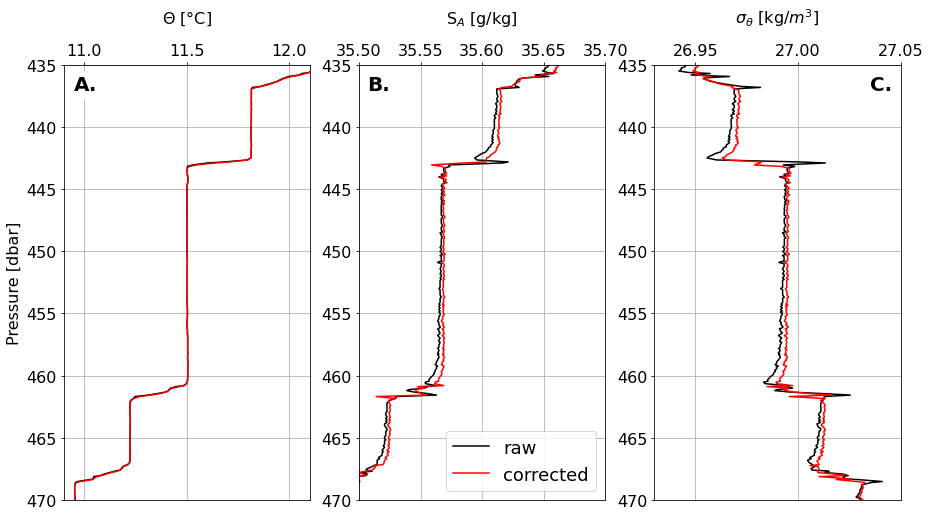
\includegraphics[width = \linewidth]{Fig12_f9139_P52_corr.png}
%	\caption{Same as in Figure \ref{fig: alamo_example} (black). Superimposed are the corrected (\textbf{A.}) conservative temperature, (\textbf{B.}) absolute salinity, and (\textbf{C.}) potential density anomaly (red)}
%	\label{fig: alamo_corrected}
%\end{figure}

The validity of the thermal inertia correction across a range of profiling speeds is assessed using an Argo float profiling in the sub-Arctic North Atlantic. The float was set to profile at different speeds, ranging from 3 cm/s to 20 cm/s. Figure \ref{fig: argo_examples} shows the effect of the dynamic correction algorithm at four different speeds.  While the amplitude of the correction is relatively small, due to the small temperature gradient, the corrected salinity does demonstrate reduced spiking at the interface (particularly visible at higher speeds), and a more homogeneous mixed layer over both shorter and longer timescales.

\begin{figure}[t]
	\centering
	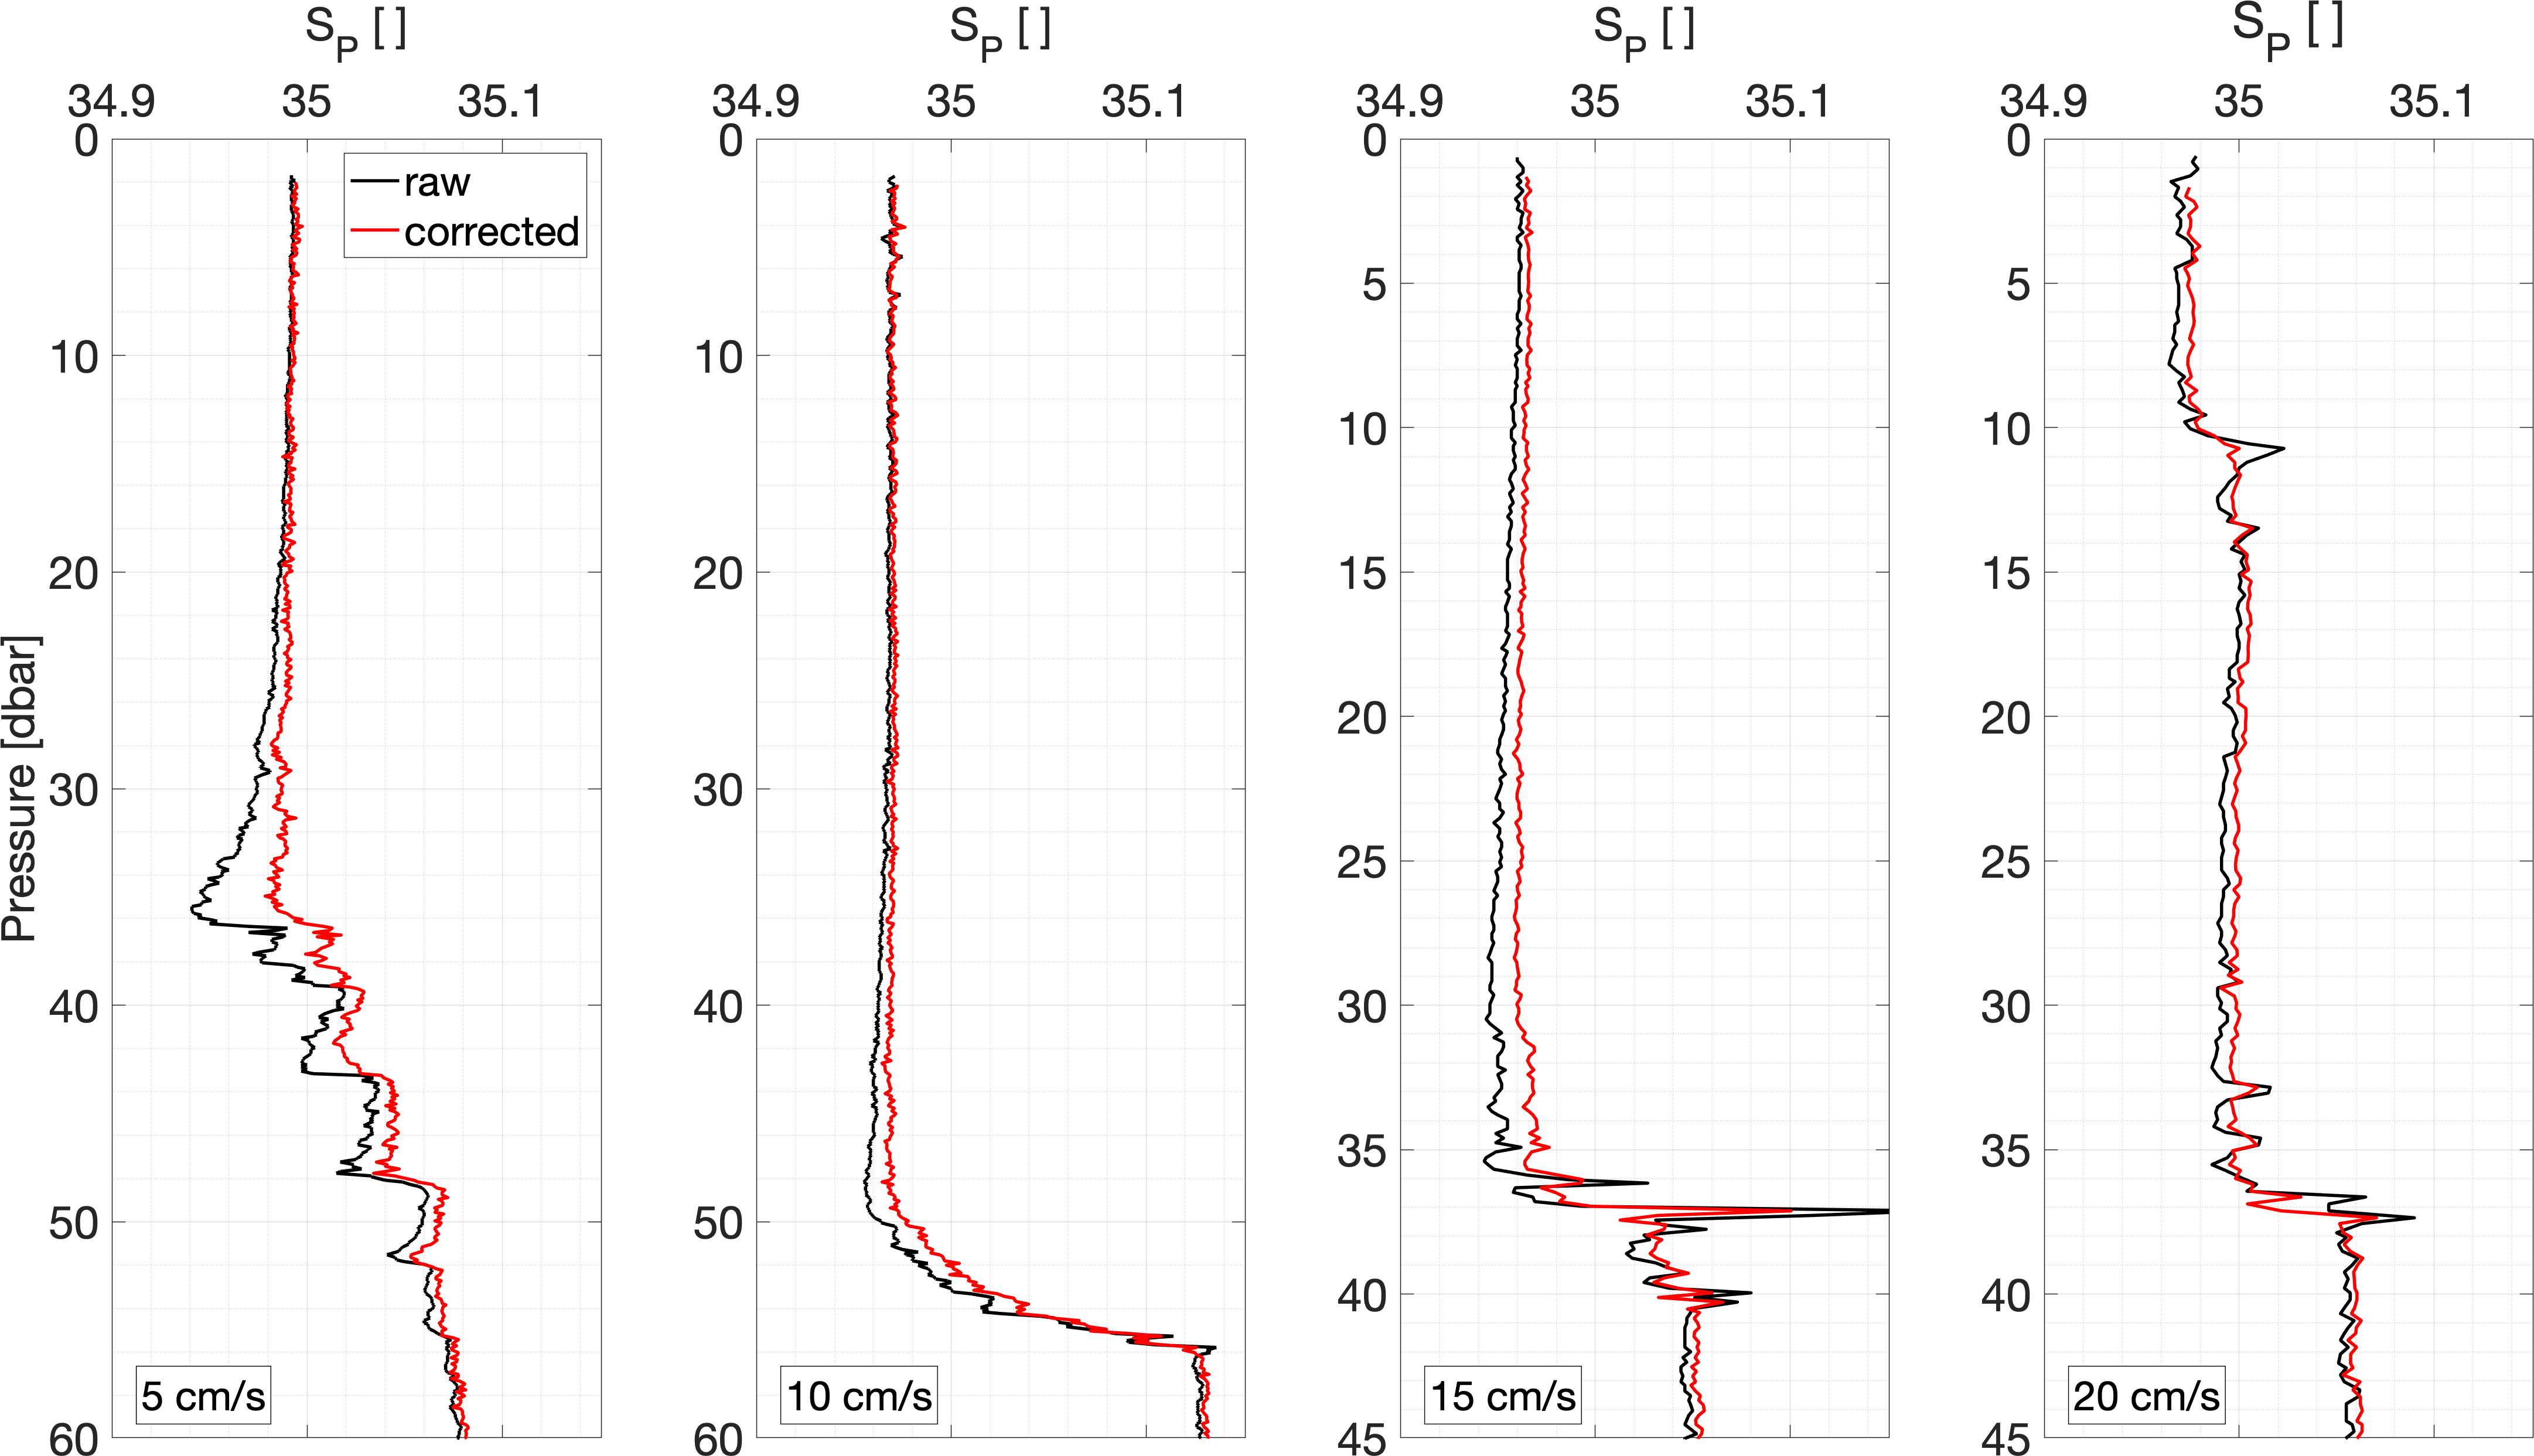
\includegraphics[width=.95\linewidth]{Fig13_Arcticfloat}\\

	\caption{Profile of practical salinity collected by float WMO4903275 at different profiling speeds as the float crosses a 1.5 to 2 $^\circ$C temperature gradient.  Raw data are shown in black, while data corrected for dynamic errors are shown in red. }
	\label{fig: argo_examples}
\end{figure}

\section{Discussion}
\label{sec: discussion}

The accuracy of both temperature and pressure on the RBR\textit{argo}$^3$ CTD is proven to be within the expected accuracy of the Argo program \citep[$\pm$0.002 $^\circ$C and $\pm$2.4 dbar, respectively;][]{Wong_2020}, throughout the range of typical pressure experienced by a Core Argo floats (i.e.,  2,000 dbar). 

While salinity is calibrated at the factory to be within the Argo accuracy requirements at atmospheric pressure ($\pm$ 0.01 ), a salinity error is introduced as pressure increases due to the physical deformation of the conductivity cell.  
This salinity bias is known to affect both inductive and electrode-based CTDs: while a salty bias is observed at depth in the RBR\textit{argo}$^3$, the electrode-based SBE41CP reports a fresh bias at depth \citep{SBEpressure}. 
A unit-based compressibility correction to conductivity is determined using a laboratory setup where each RBR\textit{argo}$^3$ is pressurized in saltwater and a cubic correction to conductivity is derived (Figure \ref{fig: saltbladder_results}). 
The proposed correction is validated in the field and is proven to reduce the salinity bias with pressure (Figure \ref{fig: YMC_data}).

Of the nineteen RBR\textit{argo}$^3$ CTDs deployed for longer than 6 months, only one was found to drift, which has been linked to a float malfunction leading to an excessive surface time likely enabling significant biofouling to occur \citep[Figure \ref{fig: stability};][]{RBRdrift}. 
Despite the relatively short time series available (average of 1.5 year), the RBR\textit{argo}$^3$ CTD presents an encouraging long-term salinity stability with 94\% (99.8\%) of profiles within $\pm$ 0.01 (0.02)  of the reference dataset.

For a profiling platform such as Argo floats, dynamic errors can significantly affect the quality of the data. 
These errors are generated by profiling through vertical temperature gradients in the water column.
The most documented dynamic error, referred to as the C-T lag, is the result of a difference in the inherent time-response of the thermistor with respect to the conductivity cell, as well as any physical distance between the location of the two sensors \citep{Horne_1980,  Lueck_1990b}. 
A robust statistical analysis based on existing literature \citep{Barth_1996,  Dever_2020} determines that an optimal lag of 0.35 s helps minimize salinity spiking for the RBR\textit{argo}$^3$ CTD.  
The absence of fall-rate dependence on the C-T lag demonstrates that the thermistor and conductivity cell are relatively well-aligned in space, thus minimizing the advective component of the C-T lag (Figure \ref{fig: CT_lag}). 
The value determined here compares well with previous estimate obtained in \cite{Halverson_2020a} using a different method. 
This empirically estimated C-T lag also agrees with the theoretical value. The response time stated by the manufacturer of the thermistor used on the RBR\textit{argo}$^3$ CTD is around 0.70 s. 
If the conductivity measurement is assumed to be instantaneous, then a lag of 0.35 s would be expected to best align the temperature to the conductivity and minimize salinity spiking. 
Some minimal spiking would remain, however, due to the fact that the temperature signal would be smoother than the conductivity readings, as it is clearly observed in Figure \ref{fig: WHOI_tank}. 
This remaining error can be mitigated by smoothing the conductivity signal, or by applying a sharpening algorithm to the temperature, as suggested in \cite{Halverson_2020a}. 
Inferring an unresolved high-frequency signal is a highly subjective task and is thus left to the discretion of the data user. 
The uncertainty in the optimal C-T lag obtained from the distribution in Figure \ref{fig: CT_lag} inevitably leads to an uncertainty in the corrected salinity. The magnitude of the propagated error is directly proportional to the temperature gradient and the ascent rate. 
As an example, a temperature gradient of 1$^\circ$C/m sampled at an ascent rate of 10 cm/s leads to a gradient of 0.1$^\circ$C/s. The standard deviation in the determined optimal C-T lag ($\sigma$=0.003 s) thus generates an error of about 3$\times$10$^{-4}$ $^\circ$C,  leading to an error in salinity of approximatively 3$\times$10$^{-4}$.

Thermal inertia errors affecting salinity from the RBR\textit{argo}$^3$ CTD exhibit two separate timescales.
The long-term thermal inertia error has a timescale $\mathcal{O}$(120 s), and generates an error on salinity about four times smaller than its short-term counterpart (Figure \ref{fig: TM_errors}).  
The correction for this second-order thermal inertia error is based on the direct measurement of the instantaneous temperature difference between the inside of the conductivity cell and the marine temperature.
Implementing the correction as a function of the temperature difference presents key advantages: First, it does not require an explicit timescale, as the timescale is implicitly included in the temperature gradient.  Second, it prevents the propagation of spurious measurement anomalies throughout the time series, as a recursive filter like L\&P90 would.
And third, being an instantaneous correction, it has significant operational advantages as implementing the correction on board autonomous platforms such as Argo floats is greatly simplified.
Just like the C-T lag, the uncertainty associated with the parameter $\text{ctcoeff}$ that propagates onto the computed salinity can be estimated by considering once more a temperature gradient of 0.1$^\circ$C/s sampled at 10 cm/s. 
The propagated uncertainty on the salinity correction from the long-term thermal inertia correction is $<$1$\times$10$^{-3}$ .

A short-term error is observed on a timescale of 5 to 10 s, and is corrected for using the L\&P90 recursive model. 
As suggested in \cite{Morison_1994}, the correction is applied by inferring the temperature of the sampled volume based on the marine temperature history (see Equation \ref{eq: LP}). 
The amplitude of the correction on the salinity is thus both temperature and salinity dependent, and is dictated by the $a$ parameter in Equation \ref{eq: LP2} (see Figure \ref{fig: TM_errors}).  
The uncertainty of the correction using the L\&P90 model is difficult to estimate, as it first requires estimating a timescale of the adjustment (i.e., $\tau$), and a corresponding amplitude ($\alpha$). 
Additionally, these two parameters have been observed to be inter-dependent \citep{Morison_1994, Lueck_1990b, Martini_2019}, suggesting than the uncertainty associated with the inferred timescale also affects the amplitude of the correction.  
Finally, the L\&P90 model being a recursive filter, the error in the correction associated with the model's parameters uncertainty accumulates through time. 

\begin{figure}[t]
	\centering
	\includegraphics[width=.95\linewidth]{Fig14_TM_error_amplitudes}\\
	\caption{Amplitude of the salinity error (in 1/$^{\circ}$C) corrected by (\textbf{A.}) the short-term, and (\textbf{B.}) the long-term thermal inertia corrections, as a function of the measured temperature and salinity.}
	\label{fig: TM_errors}
\end{figure}

For comparison, the amplitude of the short-term thermal inertia correction on the RBR\textit{argo}$^3$ is about three times smaller than the corrections currently applied to CTD data collected from an SBE41CP, and operates over similar timescales \citep{Johnson_2007}. While the long-term thermal inertia correction on the RBR\textit{argo}$^3$ has a comparable amplitude to the short-term correction, its longer timescales implies that the error is smeared over a larger part of the profiles. In particular, profiles collected in tropical waters would be more affected by thermal inertia errors due to the temperature gradients in these regions, often characterized by deeper and sharper temperature gradients.  The total amplitude of thermal inertia corrections on the RBR\textit{argo}$^3$ is highly dependent on the vertical temperature structure of the water column and is therefore difficult to characterize theoretically.  An example of the amplitude of each thermal inertia correction is shown in Figure \ref{fig: TM_errors_float} using the high-resolution data returned by the float for a short period of time (See Table \ref{app: datasets}).  As expected,  the maximum amplitude of the thermal inertia correction on a RBR\textit{argo}$^3$ is weaker than on the SBE41CP, but the correction affects a larger portion of the water column, due to the long-term component of the thermal inertia. 

\begin{figure}[t]
	\centering
	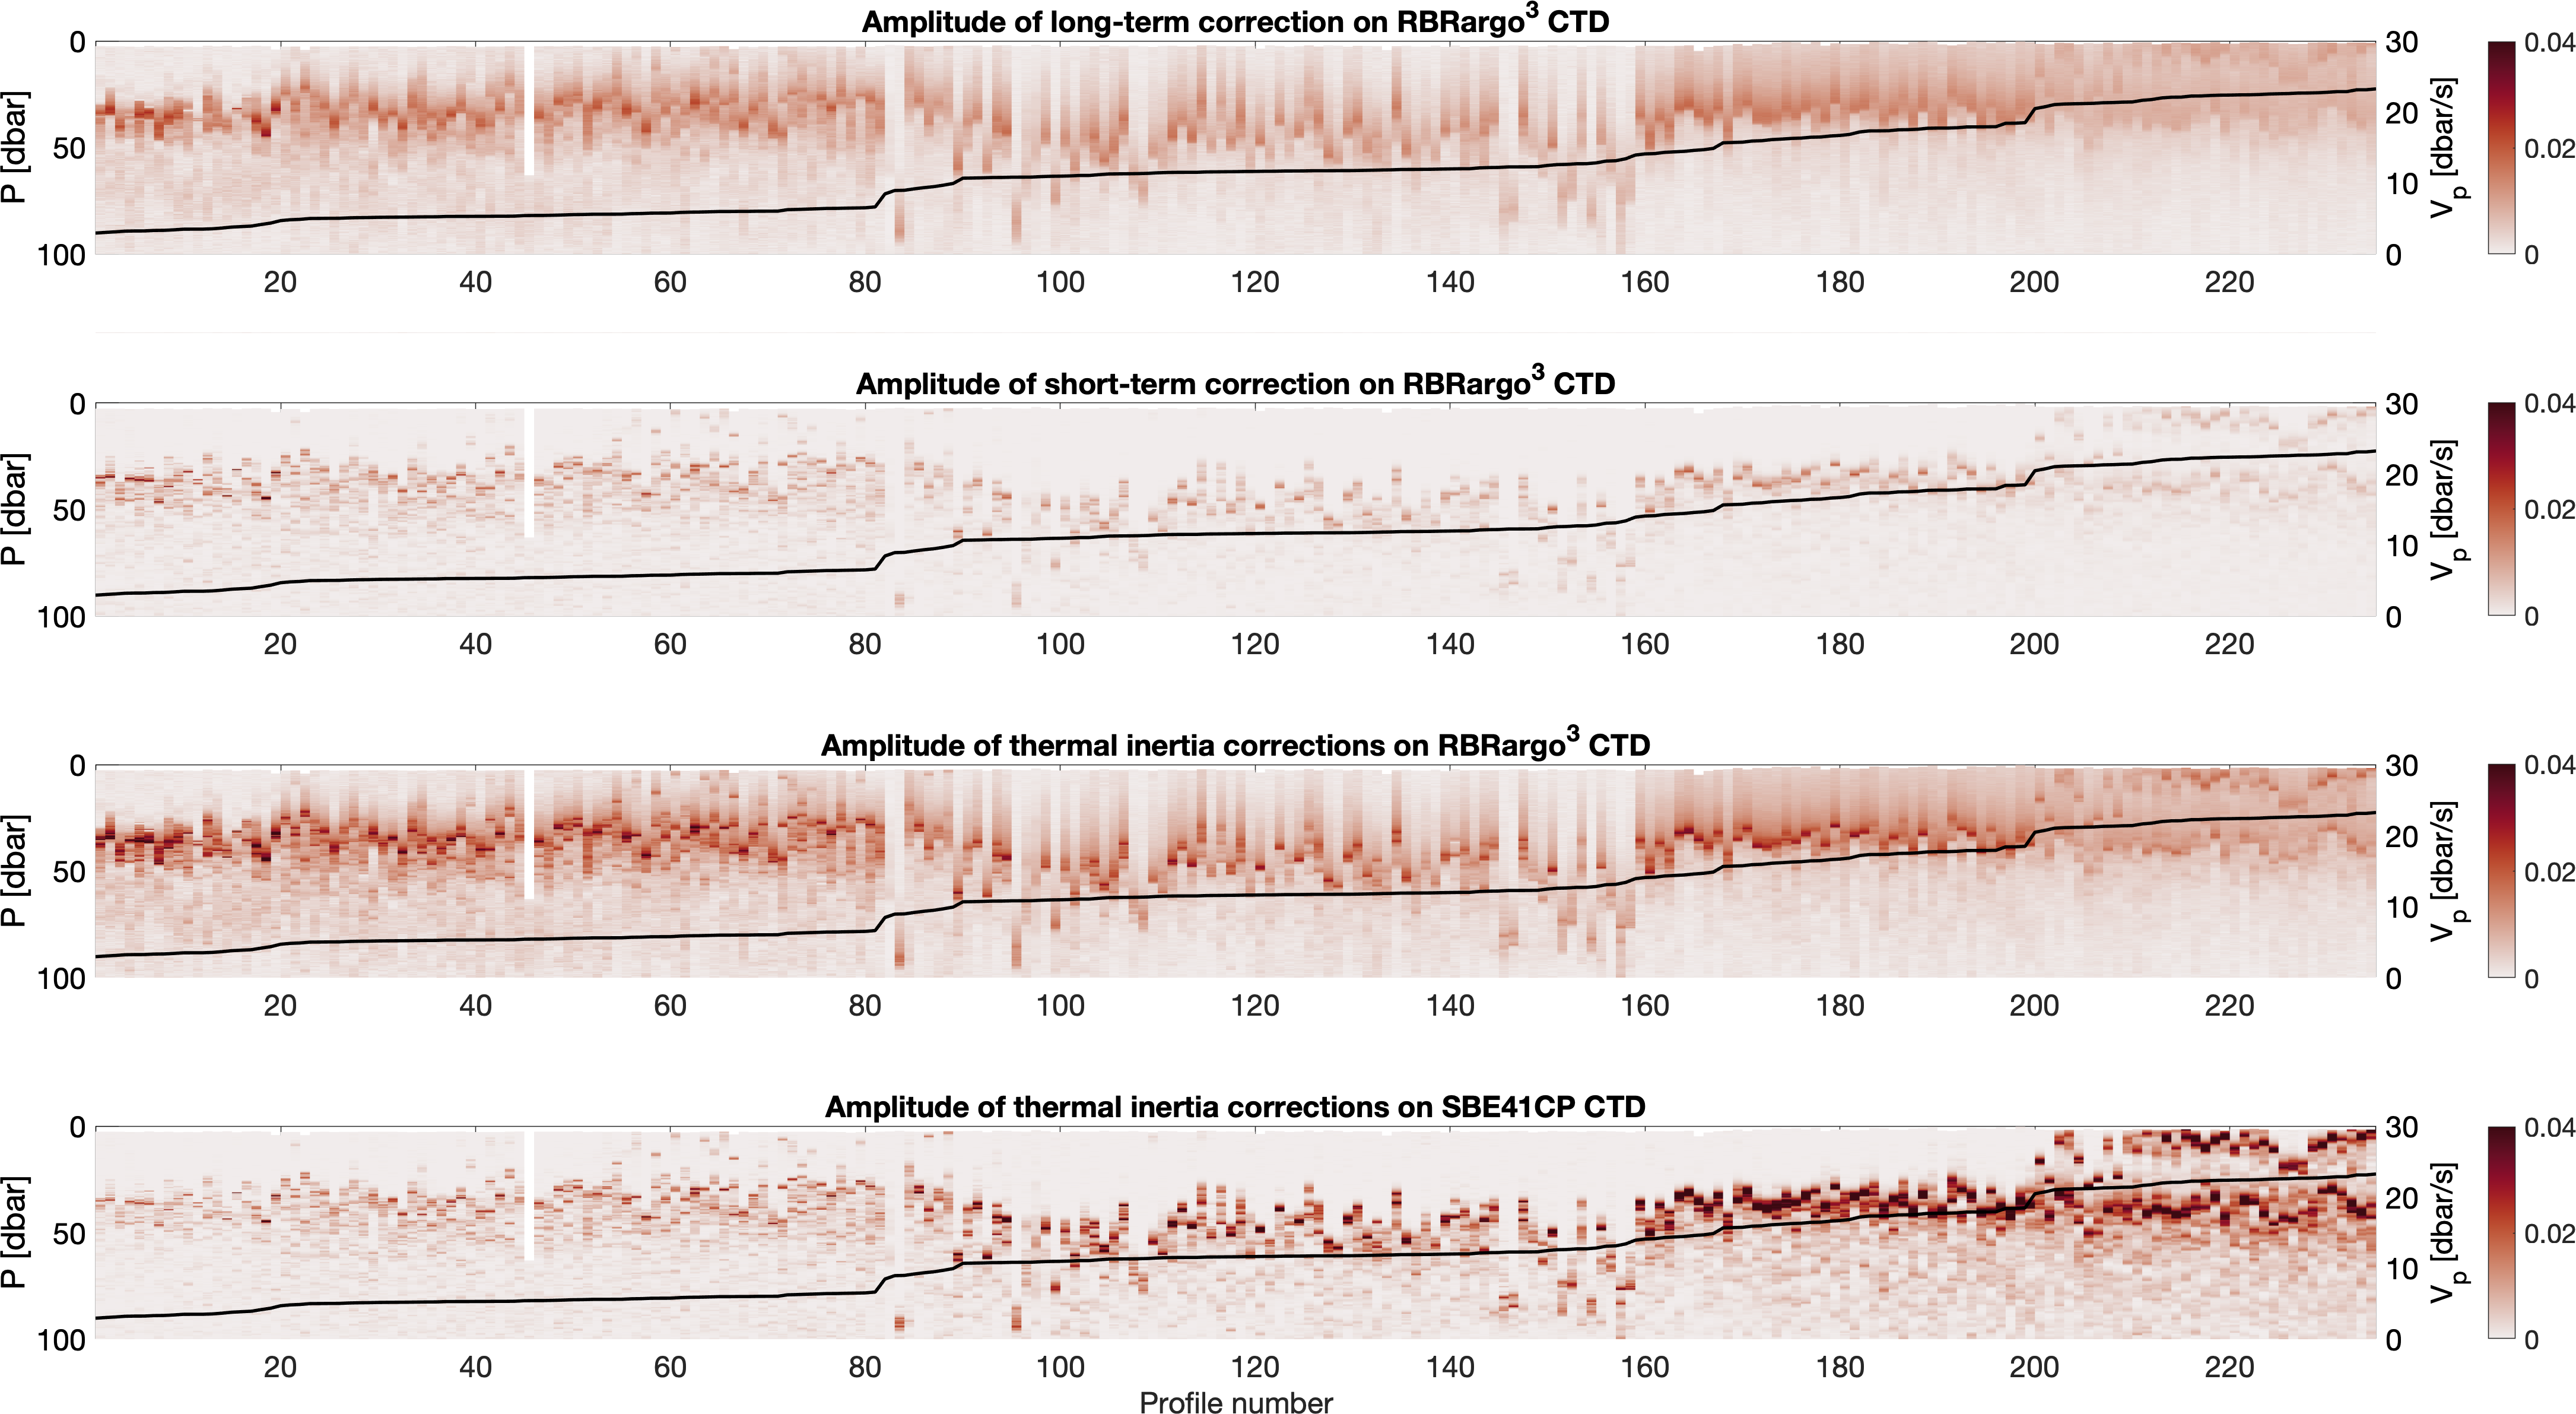
\includegraphics[width=.95\linewidth]{Fig14_SBE_vs_RBR_thermal_mass}\\
	\caption{Amplitude of the salinity correction for thermal inertia determined from high-resolution profiles collected by WMO4903275 at the base of the mixed layer.(first row) long-term correction on an RBR\textit{argo}$^3$ , (second row) short-term correction on an RBR\textit{argo}$^3$, (third row) total thermal inertia correction on an RBR\textit{argo}$^3$,  and (fourth row) total thermal inertia correction for a SBE41CP \citep{Johnson_2007}. Profiles are organized by increasing profiling speed $V_p$.}
	\label{fig: TM_errors_float}
\end{figure}

Because thermal inertia errors are generated from the heat exchange between the conductivity cell and its surrounding water, the thermal inertia corrections derived in this study are expected to be a function of the profiling speed.  
The range of speeds explored in the flume not only encompasses the nominal speed for Argo floats ($\sim$ 10 cm/s), but also covers the realistic range of speeds an autonomous profiling platform can achieve (e.g., floats, gliders). 
The relationship linking the three coefficients to profiling speed are modelled using a power-law, as the theoretical work from \cite{Lueck_1990a} suggests, but it is not intended to be anything more than an empirical fit. 
Caution should be used when extrapolating coefficients outside of the range of explored speeds, such as for typical CTD rosette profiling speeds (e.g., 100 cm/s).  

One of the most important results of the dependence on flow-rate is the fact that, due to the shape of the power-law function, the three coefficients are not only weaker, but they are also less dependent on the profiling speed (Figure \ref{fig: TM_vs_speed}).
The main consequence is that the thermal inertia correction is thus less sensitive to uncertainties in both coefficients and flow-rates when profiling at higher speeds.
To minimize the uncertainty on the thermal inertia correction, it is therefore recommended to profile at higher speeds, which could be compensated with a higher sampling rate to preserve vertical resolution.
This can be directly observed in Figures \ref{fig: argo_examples} and \ref{fig: TM_errors_float}, where the salinity error visible in the raw in-situ data is clearly smaller at faster speeds, despite crossing a similar temperature gradient (1.5 to 2$^\circ C$).

For an RBR\textit{argo}$^3$ profiling at approximatively 10 cm/s the best practices for dynamic correctioncan be summarized as: (1) lagging the temperature signal by -0.35 s, (2) correcting for the long-term thermal inertia error using Equation \ref{eq: long-term_TM} and ctcoeff = $9.7\times10^{-3}$, and (3) correcting for the short-term thermal inertia error using L\&P90 (Equations \ref{eq: LP} and \ref{eq: LP2}) with $\alpha$ = 0.041 and $\tau$ = 8.11s.

%%%%%%%%%%%%%%%%%%%%%%%%%%%%%%%%%%%%%%%%%%%%%%%%%%%%%%%%%%%%%%%%%%%%%
% TABLES---INSERT NEAR IN-TEXT DISCUSSION
%%%%%%%%%%%%%%%%%%%%%%%%%%%%%%%%%%%%%%%%%%%%%%%%%%%%%%%%%%%%%%%%%%%%%
%%  Enter tables near where they are discussed within the document. 
%%  Please place tables before/after paragraphs, not within a paragraph.
%%
%
%\begin{table}[t]
%\caption{This is a sample table caption and table layout.  Enter as many tables as
%  necessary at the end of your manuscript. Table from Lorenz (1963).}\label{t1}
%\begin{center}
%\begin{tabular}{ccccrrcrc}
%\hline\hline
%$N$ & $X$ & $Y$ & $Z$\\
%\hline
% 0000 & 0000 & 0010 & 0000 \\
% 0005 & 0004 & 0012 & 0000 \\
% 0010 & 0009 & 0020 & 0000 \\
% 0015 & 0016 & 0036 & 0002 \\
% 0020 & 0030 & 0066 & 0007 \\
% 0025 & 0054 & 0115 & 0024 \\
%\hline
%\end{tabular}
%\end{center}
%\end{table}

%%%%%%%%%%%%%%%%%%%%%%%%%%%%%%%%%%%%%%%%%%%%%%%%%%%%%%%%%%%%%%%%%%%%%
% FIGURES---INSERT NEAR IN-TEXT DISCUSSION
%%%%%%%%%%%%%%%%%%%%%%%%%%%%%%%%%%%%%%%%%%%%%%%%%%%%%%%%%%%%%%%%%%%%%
%%  Enter figures near where they are discussed within the document.
%%  Please place figures before/after paragraphs, not within a paragraph.
% %
%
%\begin{figure}[t]
%  \noindent\includegraphics[width=19pc,angle=0]{figure01.pdf}\\
%  \caption{Enter the caption for your figure here.  Repeat as
%  necessary for each of your figures. Figure from \protect\cite{Knutti2008}.}\label{f1}
%\end{figure}

\clearpage
%%%%%%%%%%%%%%%%%%%%%%%%%%%%%%%%%%%%%%%%%%%%%%%%%%%%%%%%%%%%%%%%%%%%%
% ACKNOWLEDGMENTS
%%%%%%%%%%%%%%%%%%%%%%%%%%%%%%%%%%%%%%%%%%%%%%%%%%%%%%%%%%%%%%%%%%%%%
\acknowledgments
%  Keep acknowledgments (note correct spelling: no ``e'' between the ``g'' and
% ``m'') as brief as possible. In general, acknowledge only direct help in
%  writing or research. Financial support (e.g., grant numbers) for the work done, 
%  for an author, or for the laboratory where the work was performed must be 
%  acknowledged here rather than as footnotes to the title or to an author's name.
%  Contribution numbers (if the work has been published by the author's institution 
%  or organization) should be placed in the acknowledgments rather than as 
%  footnotes to the title or to an author's name.

Drs. Owens and Richards contributed to the characterization of the thermal inertia errors. Dr. Wijffels lead the validation of pressure and temperature measurements on a RBR\textit{argo}$^3$. Dr. Wong conducted the analysis of salinity measurement stability. Drs. Shkvorets, Halverson, and Johnson provided support in the experimental design and analysis of the compressibility error in salinity. Thanks go to the Argo community at large, for their support in facilitating deployments of RBR\textit{argo}$^3$ CTDs,  in providing ancillary datasets, and in offering feedback on the analysis. Special thanks are directed to the ``Argo RBR Data Task Team", specially formed to collaborate on the analysis of the RBR\textit{argo}$^3$. 

%%%%%%%%%%%%%%%%%%%%%%%%%%%%%%%%%%%%%%%%%%%%%%%%%%%%%%%%%%%%%%%%%%%%%
% DATA AVAILABILITY STATEMENT
%%%%%%%%%%%%%%%%%%%%%%%%%%%%%%%%%%%%%%%%%%%%%%%%%%%%%%%%%%%%%%%%%%%%%
% 
%
\datastatement
%  The data availability statement is where authors should describe how the data underlying 
%  the findings within the article can be accessed and reused. Authors should attempt to 
%  provide unrestricted access to all data and materials underlying reported findings. 
%  If data access is restricted, authors must mention this in the statement. See
%  {http://www.ametsoc.org/PubsDataPolicy} for more info.

The data used in this work is available in a dedicated GitHub repository: \url{https://github.com/matdever/RBRargo3_paper}. The code necessary to produce the displayed figures are also included in the repository.

%%%%%%%%%%%%%%%%%%%%%%%%%%%%%%%%%%%%%%%%%%%%%%%%%%%%%%%%%%%%%%%%%%%%%
% APPENDIXES
%%%%%%%%%%%%%%%%%%%%%%%%%%%%%%%%%%%%%%%%%%%%%%%%%%%%%%%%%%%%%%%%%%%%%

\appendix[A]
\appendixtitle{Datasets}
\label{app: datasets}

\begin{table}[h!]
	\centering
	\caption{\label{tab: cruise_data}List of the datasets obtained from field cruises used to characterize the RBR\textit{argo}$^3$. }
\begin{tabular}{|l|l|l|l|l|l|l|}
	\hline
Cruise name 	& Partner Institution					& Year 	& Ocean basin           		& RBR\textit{argo}$^3$ S/Ns 										\\ \hline
Line P      			& DFO Canada 							& 2018 & Northeast Pacific Ocean     	& 060672                        						\\
JAMSTEC     	& JAMSTEC             						& 2018 & Northwest Pacific Ocean    	& 060669, 060671                				\\
PEACH       		& WHOI     									& 2018 & Northwestern Atlantic Ocean& 060667, 060668, 060671					\\
AR41        			& WHOI     									& 2019 & Northwestern Atlantic Ocean& 060667, 060668, 060670        			\\
YMC         		& CSIRO/WHOI               						& 2019 & Southeastern Indian Ocean           		&	060669, 060671								\\ \hline
\end{tabular}
\footnotesize
\raggedright
\\DFO = Department of Fisheries and Ocean\\
JAMSTEC = Japan Agency for Marine-Earth Science and Technology\\
WHOI = Woods Hole Oceanographic Institution\\
CSIRO = Commonwealth Scientific and Industrial Research Organisation.
\end{table}

\begin{table}[h!]
	\centering
	\caption{\label{tab: float_data}List of the datasets obtained from profiling floats used to characterize the RBR\textit{argo}$^3$. }
\begin{tabular}{|l|l|l|l|l|l|}
	\hline
Float type & Float ID & Data resolution & Institution					& Year & Ocean basin           \\ \hline
ALAMO & 9139 & 1 Hz & WHOI & 2017 & Caribbean Sea \\
Argo float & WMO4903275 & 0.10 dbar bins & WHOI & 2020 & North Atlantic \\ \hline
\end{tabular}
\footnotesize
\raggedright
\\WHOI = Woods Hole Oceanographic Institution\\
\end{table}


\appendix[B]
\appendixtitle{Calibration of rosette data}
\label{app: Kfactor}

Similar to SBE911 cross-calibration protocol, bottle salinity samples collected from the CTD rosette can be used to cross-calibrate RBR\textit{argo}$^3$ CTDs mounted on a shipboard rosette. Inductive conductivity cells, like the one on the RBR\textit{argo}$^3$, are subject to the proximity effect: Any material located within a 15 cm radius from the conductivity cell would affect measurements of conductivity in a multiplicative way \citep{Halverson_2020}. The multiplicative factor is named the K-factor:
\begin{equation}
	C = K \times C_{raw}
	\label{eq: Kfactor_fit}
\end{equation}

 A conductive material, such as a metal, would generate a K-factor smaller than 1 (i.e., the apparent conductivity would appear larger than the one of the water), while an insulating material such as plastic would lead to a K-factor greater than 1 (i.e., the apparent conductivity would appear smaller than the one of the water). The two RBR\textit{argo}$^3$ CTDs mounted on the rosette during the YMC cruise onboard the RV Investigator in 2019 \citep[serial numbers 060669 and 060671;][]{YMCreport_2019} are cross-calibrated with salinity water samples measured using an AutoSal Guildline using a zero-intercept linear fit (see Equation \ref{eq: Kfactor_fit}). A K-factor of 1.0001 and 0.9997 are obtained for SN060669 and SN060671, respectively.

%%%%%%%%%%%%%%%%%%%%%%%%%%%%%%%%%%%%%%%%%%%%%%%%%%%%%%%%%%%%%%%%%%%%%
% REFERENCES
%%%%%%%%%%%%%%%%%%%%%%%%%%%%%%%%%%%%%%%%%%%%%%%%%%%%%%%%%%%%%%%%%%%%%
% Make your BibTeX bibliography by using these commands:
\bibliographystyle{ametsocV6}
\bibliography{RBRargo3}


\end{document}